\documentclass{article}
\usepackage{iclr2026_conference,times}
\input{math_commands.tex}
\usepackage{hyperref}
\usepackage{url}

\usepackage{graphicx}
\usepackage{subcaption}
\usepackage[export]{adjustbox}
\usepackage{booktabs}
\usepackage{float}
\usepackage{tabularx}
\usepackage{makecell}
\usepackage{ragged2e}
\usepackage{listings}

\lstset{
    basicstyle=\scriptsize\ttfamily,
    breaklines=true,
    frame=single,
    captionpos=b
}

\title{Artifact-Driven Metadata Schema Development: A Human-in-the-Loop Methodology with Multimodal LLMs}

\author{AJ Carl P. Dy$^{\dagger}$ \& Aivin V. Solatorio$^{*}$ \\
Development Data Group \\
Office of the World Bank Group Chief Statistician \\
The World Bank \\
1818 H Street N.W., \\
Washington, 20433 \\
District of Columbia, USA \\
\texttt{\{ady, asolatorio\}@worldbank.org} }

\iclrfinalcopy % Uncomment for camera-ready version, but NOT for submission.
\begin{document}

\maketitle

\begingroup
\renewcommand\thefootnote{\fnsymbol{footnote}}
\footnotetext[2]{GitHub/HF: \href{https://github.com/ajdajd}{\texttt{@ajdajd}}, \href{mailto:ajcarl.dy@gmail.com}{ajcarl.dy@gmail.com}}
\footnotetext[1]{GitHub/HF: \href{https://github.com/avsolatorio}{\texttt{@avsolatorio}}, \href{mailto:avsolatorio@gmail.com}{avsolatorio@gmail.com}}
\endgroup

\begin{abstract}

Developing an operational metadata schema for a multimodal artifact class requires identifying its descriptive requirements before metadata extraction can begin. We present an artifact-driven, human-in-the-loop methodology that adapts principles from metadata profile development, schema discovery, ontology learning, and multimodal document understanding. The methodology decomposes schema development into explicit, evidence-preserving semantic transformations connected by intermediate knowledge artifacts. Multimodal large language models support artifact interpretation, concept synthesis, and constrained semantic comparison, while human experts determine conceptual boundaries, operational fields, and schema revisions. We apply the methodology to 210 data snapshots extracted from institutional documents, producing the 36-field Data Snapshot Metadata Schema, which is subsequently evaluated against a separate collection of 202 snapshots. The contribution is a structured adaptation of established methods to the input and output conditions of this problem: multimodal artifacts as evidence and an operational metadata schema as the endpoint.

\end{abstract}

\section{Introduction}

Metadata provides the descriptive foundation that enables digital resources to be organized, discovered, exchanged, and reused~\citep{gilliland2008}. Well-designed metadata schemas support consistent annotation, interoperability, retrieval, provenance tracking, and downstream analytical workflows across heterogeneous information systems~\citep{metadatainteroperability2006}. For mature domains, such schemas typically emerge through years of community collaboration, iterative refinement, and the gradual convergence of expert knowledge into widely adopted metadata standards~\citep{caplan2003}.

Recent advances in document understanding and multimodal information systems have made it increasingly feasible to extract analytical artifacts embedded within documents—such as statistical tables, charts, maps, dashboards, and monitoring frameworks—as standalone information objects that can be indexed, retrieved, and managed independently of their source documents~\citep{wang2025,dy2026}. As these artifacts become standalone information objects, they require metadata describing their analytical content, structure, and context, rather than solely the bibliographic properties of the documents from which they originate~\citep{gilliland2008}. While existing metadata standards provide many relevant concepts, no single standard adequately describes the metadata required to represent the analytical semantics of many such artifact types~\citep{gilliland2008}.

Our broader research investigates one such class of artifacts, which we refer to as \emph{data snapshots}: semantically meaningful analytical artifacts extracted from institutional documents and managed as independent information objects~\citep{dy2026}. Developing a metadata extraction and retrieval pipeline for these artifacts required a metadata schema capable of describing the snapshots themselves rather than only their source documents.

Existing metadata standards provide many concepts relevant to digital resources, but at the outset of this work no dedicated operational metadata schema or directly adoptable metadata profile had been identified for data snapshots as defined here~\citep{gilliland2008,metadatainteroperability2006}. Before metadata could be extracted systematically, relevant concepts therefore had to be selected, supplemented, and organized into an artifact-specific specification. This raised a more fundamental question: how can an initial operational metadata schema be systematically developed when the descriptive requirements of the artifact class have not yet been consolidated?

Developing an initial metadata schema for a previously unsupported artifact type remains largely expert-driven. The process requires discovering candidate metadata concepts from representative artifacts, consolidating semantically related concepts, refining conceptual boundaries, and translating the resulting concept inventory into an operational metadata schema through iterative expert review~\citep{greenberg2005,coyle2009applicationprofiles}. Existing research on metadata standardization, schema discovery, ontology engineering, and ontology learning provides complementary foundations for this task. The question addressed here is how those foundations can be adapted when the descriptive requirements must first be discovered from multimodal artifacts and the required endpoint is an operational metadata schema.

Recent advances in multimodal large language models (LLMs) provide an opportunity to support the exploratory stages of metadata schema development~\citep{ding2026vrdu,bian2025}. Rather than treating schema development as a single prompting task, we propose a human-in-the-loop methodology that decomposes the process into explicit semantic transformations connected by intermediate knowledge artifacts. These artifacts preserve evidence for expert review while enabling multimodal LLMs and human experts to contribute complementary forms of reasoning throughout the workflow.

We demonstrate the methodology through the development of the Data Snapshot Metadata Schema for data snapshots. The case study shows how heterogeneous metadata observations can be progressively transformed into an operational metadata schema through explicit intermediate knowledge artifacts that support transparent human–LLM collaboration. Beyond the resulting schema, the paper contributes a repeatable methodology for developing metadata schemas for previously unsupported classes of multimodal analytical artifacts.

\section{Related work}

The proposed methodology adapts established ideas from metadata profile development, schema discovery, ontology learning, knowledge graph construction, and multimodal document understanding. It integrates these strands into a workflow for deriving an operational metadata schema from the multimodal artifacts it is intended to describe. Specifically, the methodology connects independently gathered artifact evidence to a shared concept inventory and, ultimately, an operational metadata schema while preserving traceability to each source artifact.

\subsection{Metadata standards and schema development}

Metadata standards provide descriptive frameworks through which digital resources can be organized, discovered, exchanged, and preserved~\citep{gilliland2008}. Application-profile guidance further distinguishes the characterization of the resources being described, the selection and definition of metadata terms, the design of metadata records and constraints, and the documentation of usage rules~\citep{coyle2009applicationprofiles}. These activities provide a useful foundation for operational metadata schema development.

Existing metadata vocabularies nevertheless do not remove the need for application-specific design. A target artifact class may require terms drawn from several sources, locally defined terms, constraints, and usage guidance assembled into a coherent operational specification~\citep{greenberg2005,coyle2009applicationprofiles}. The problem addressed here is therefore not the absence of relevant metadata concepts, but the absence, at the outset of the work, of a directly adoptable metadata schema for data snapshots as defined in this study.

The resulting Data Snapshot Metadata Schema is presented as a dedicated operational specification for this artifact class rather than as a community standard. Standards alignment, community governance, and formal standardization are separate, longer-term processes beyond the artifact-driven development studied here.

\subsection{LLM-assisted schema discovery and ontology learning}

LLMs4SchemaDiscovery presents an iterative human-in-the-loop workflow for deriving scientific schemas from text through seed-schema construction, expert feedback, corpus expansion, and ontology grounding~\citep{sadruddin2025schemadiscovery}. Our setting differs in both input modality and workflow organization: schema evidence is derived from multimodal analytical artifacts, observations are generated independently for each snapshot, and deterministic field profiles aggregate local evidence before concepts are consolidated.

LLM-assisted ontology learning provides a second methodological foundation. LLMs4OL decomposes ontology learning into tasks such as term typing, taxonomy discovery, and non-taxonomic relation extraction~\citep{giglou2023llms4ol}. NeOn-GPT embeds LLM prompting within a staged ontology-development methodology and produces formal ontologies from domain descriptions and competency questions~\citep{fathallah2025neongpt}; its extended version adds ontology reuse together with automated verification and repair~\citep{fathallah2026extended}. OntoGenix similarly provides a structured dataset-to-ontology workflow that includes ontology planning and construction as well as mappings and RDF generation~\citep{valcalvo2025ontogenix}.

Together, these studies show how LLMs can support progressively more formal knowledge-representation tasks, from term typing and taxonomy construction to ontology reuse, verification, and repair.

Stage-wise evidence suggests that expert involvement becomes increasingly important as ontology work progresses from term extraction toward hierarchy and relation specification~\cite{ding2026ontology}. A systematic review similarly identifies broad use of LLMs across ontology-engineering activities alongside limited human evaluation and inconsistent validation practices~\cite{li2026ontologyreview}. These findings support assigning exploratory discovery and abstraction to the LLM while retaining human responsibility for conceptual boundaries, consolidation decisions, and operational schema design.

\subsection{Open schema induction and knowledge graph construction}

Open knowledge graph construction offers related patterns for discovery, definition, and canonicalization. The Extract--Define--Canonicalize framework extracts relations from text, defines candidate relations, and canonicalizes them against an existing or induced schema~\citep{zhang2024edc}. Broader surveys place these operations within LLM-supported ontology engineering, information extraction, schema induction, and knowledge integration~\citep{bian2025}. These approaches support open discovery and semantic consolidation, but primarily target relational schemas and knowledge graphs rather than an operational metadata specification for describing multimodal artifacts.

\subsection{Multimodal document understanding}

Multimodal document-understanding research provides the capabilities required to interpret combinations of text, tables, charts, layout, and other visual evidence in visually rich documents~\citep{wang2025,ding2026vrdu}. Its usual objective is to understand or extract information from documents, often with a predefined target representation. In this work, multimodal interpretation is instead used upstream to discover which metadata concepts are needed: the visual artifacts are evidence from which the descriptive representation is derived.

\subsection{Positioning of this work}

Taken together, the reviewed literature provides human-in-the-loop schema discovery, staged ontology construction, task decomposition, open schema induction and canonicalization, and multimodal artifact interpretation. This paper adapts these strands into an artifact-driven architecture for metadata schema development. The architecture analyzes snapshots independently before introducing a shared vocabulary; retains local observations rather than immediately absorbing them into an evolving schema; aggregates evidence in deterministic field profiles; separates canonical concept synthesis, expert refinement, and concept coverage assessment; and subsequently translates the refined concept inventory into an operational metadata schema. Each transformation remains traceable to the visual artifacts that motivated it.

Table~\ref{tab:positioning} summarizes the methodological contributions adopted from each literature group and the corresponding differences in this work.

\begin{table}[!ht]
    \centering
    \caption{Comparison of the proposed artifact-driven methodology with representative prior work.}
    \label{tab:positioning}
    \renewcommand{\arraystretch}{1.4}
    \newcolumntype{Y}[1]{>{\hsize=#1\hsize\raggedright\arraybackslash}X}
    \small
    \begin{tabularx}{\textwidth}{Y{0.95} Y{1.025} Y{1.025}}
    \toprule
        \textbf{Literature group} & \textbf{Relevant contribution} & \textbf{Distinction from this work} \\
        \midrule
        LLMs4SchemaDiscovery & Human-in-the-loop schema discovery and refinement & Scientific text input and direct mutation of an evolving schema \\
        Ding et al. ontology study & Increasing expert responsibility during formalization & Evaluation of classical ontology stages in a healthcare case \\
        NeOn-GPT and Extended NeOn-GPT & Staged construction, reuse, verification, and repair & Formal ontology as the endpoint \\
        OntoGenix & Structured, multi-stage dataset-to-ontology workflow & Structured dataset input and ontology, mappings, and knowledge graph outputs \\
        EDC and the KG-construction survey & Open discovery, definition, canonicalization, and schema induction & Primary orientation toward knowledge graph construction \\
        LLMs4OL & Decomposition of ontology-learning tasks & Task decomposition rather than an end-to-end operational metadata-schema workflow \\
        VRDU survey & Multimodal interpretation of visual, textual, and layout information & Schema development is not the primary objective \\
    \bottomrule
    \end{tabularx}
\end{table}

\section{Conceptual framework}

This paper addresses the problem of developing metadata schemas for multimodal analytical artifact types that lack a dedicated operational metadata specification. Before presenting the proposed methodology, we establish the conceptual framework that underpins the remainder of the paper. In particular, we distinguish among \emph{metadata}, \emph{metadata concept inventory}, and \emph{metadata schema}. We then define how \emph{metadata schema development} is used in this paper and formulate the problem addressed by the methodology.

\subsection{Data snapshots as independent information objects}

A \emph{data snapshot} is a semantically meaningful analytical artifact extracted from a document page and treated as an independent information object~\citep{dy2026}. Examples include statistical tables, charts, maps, dashboards, monitoring frameworks, and composite analytical figures. Representative examples are provided in Appendix~\ref{appendix:datasnapshots}. Unlike document pages, data snapshots encapsulate specific analytical content and are often reused, searched, or interpreted independently of their source documents. Treating each data snapshot as an independent information object enables metadata to be assigned at the level where the analytical content is expressed, rather than inherited solely from the source document.

Conventional document-level metadata such as title, author, publication date, or organization provides valuable context about the source document but is insufficient to describe the analytical content of individual data snapshots. For example, multiple data snapshots within the same report may describe different indicators, geographic regions, populations, or time periods while sharing identical document metadata. Effective organization, retrieval, and downstream analysis therefore require metadata that describes the snapshots themselves rather than only the documents from which they were extracted.

\subsection{Conceptual distinctions}

Building on the definition of a data snapshot, we distinguish three closely related concepts that play distinct roles in the proposed workflow.

\paragraph{Metadata}

Metadata is descriptive information about a data snapshot. It consists of properties that help identify, interpret, organize, retrieve, or manage a snapshot~\citep{gilliland2008}. Examples include the analytical indicator represented, geographic coverage, temporal coverage, visualization type, source organization, and other descriptive attributes. Metadata primarily answers the question: "What does this snapshot represent?"

\paragraph{Metadata concept inventory}

A metadata concept inventory is the intermediate conceptual artifact used in this methodology. It records canonical metadata concepts together with definitions, rationales, representative discovered fields, and expert decisions to retain, merge, or exclude concepts. It supports conceptual consolidation and review before the concepts are translated into operational metadata fields. The inventory differs from an ontology in that it does not assert a class hierarchy, formal semantic relations, axioms, or instances~\citep{uschold&gruninger1996,noy&mcguinness2001}.

\paragraph{Metadata schema}

A metadata schema is an operational specification describing which metadata fields should be captured for a data snapshot together with their definitions, intended use, and annotation guidance~\citep{greenberg2005,coyle2009applicationprofiles}. It translates the refined metadata concept inventory into a record structure that can guide subsequent annotation, storage, retrieval, and extraction. In this paper, \emph{metadata schema development} denotes the full evidence-driven process of discovering, consolidating, specifying, and assessing these metadata fields.

Figure~\ref{fig:conceptual_relationship} summarizes the relationships among these concepts.

\begin{figure}[!ht]
    \centering
    
\includegraphics[width=0.35\linewidth]{data/conceptual_hierarchy.png}
    \caption{Relationship between data snapshots, metadata, the intermediate concept inventory, and the metadata schema. Metadata extraction and downstream applications are shown separately because they assume that an operational metadata schema already exists. [TODO: Replace the ontology node with the metadata concept inventory and show the metadata schema as its operationalization.]}
    \label{fig:conceptual_relationship}
\end{figure}

\subsection{Scope}

The proposed methodology addresses the development of an operational metadata schema for a class of multimodal analytical artifacts that lacks a dedicated operational schema or directly adoptable metadata profile. Existing standards and vocabularies may still provide applicable terms. The task is to identify, consolidate, define, and operationalize descriptive requirements grounded in representative artifacts.

As illustrated in Figure~\ref{fig:conceptual_relationship}, the operational metadata schema is the final descriptive representation produced by the methodology. Its coverage is then evaluated against held-out artifacts. Metadata extraction and downstream applications fall outside the scope of this work, as do subsequent activities that adapt the schema to specific technical or interoperability requirements.

\subsection{Problem definition}

Schema development for established resource types can draw on mature standards, shared conventions, and accumulated domain knowledge. When an artifact class is not yet adequately characterized, its descriptive requirements cannot be assumed in advance. Defining fields solely from expert expectations or a small number of salient examples may omit less frequent properties that remain important for interpretation or discovery. The schema must therefore be grounded in evidence from representative artifacts before a shared vocabulary is fixed.

We therefore consider the following problem:

\begin{quote}
Given a representative collection of multimodal analytical artifacts for which no dedicated operational metadata schema exists, how can an operational metadata schema be systematically developed from artifact-level evidence?
\end{quote}

This problem presents four challenges. First, the relevant metadata space is initially unknown. Second, artifact-level observations are heterogeneous and local; they must be aggregated and consolidated while retaining traceability to their source artifacts. Third, the resulting concept inventory must be translated into fields, definitions, and guidance suitable for consistent use. Finally, the completed schema must be evaluated on held-out artifacts without treating every rare semantic distinction as evidence for a new field.

We address these challenges by decomposing metadata schema development into a sequence of semantic transformations connected by explicit intermediate knowledge artifacts. Multimodal LLMs support artifact interpretation, broad metadata discovery, semantic consolidation, and structured gap analysis. Human experts retain responsibility for scope, conceptual boundaries, operational schema design, and the adjudication of validation evidence.

The following section presents the proposed methodology.

\section{Methodology}
\label{sec:methodology}

This section presents a reusable methodology for developing an operational metadata schema for multimodal analytical artifacts that lack an established descriptive standard. The methodology decomposes schema development into a sequence of semantic transformations connected by explicit intermediate knowledge artifacts. Multimodal LLMs support selected discovery, consolidation, and assessment tasks, while human experts retain responsibility for conceptual and operational decisions.

The stages separate artifact-level discovery, evidence aggregation, concept synthesis, expert refinement, concept coverage assessment, metadata schema design and specification, and schema validation. This decomposition makes each transformation independently reviewable and preserves traceability from the operational schema to the artifacts that motivated it. Table~\ref{tab:methodology_summary} summarizes the workflow.

\begin{table}[!ht]
    \centering
    \caption{Summary of the proposed methodology. Each stage transforms an explicit input artifact into an output that can be reviewed before the next stage.}
    \label{tab:methodology_summary}
    \renewcommand{\arraystretch}{1.4}

    \newcolumntype{Y}[1]{>{\hsize=#1\hsize\raggedright\arraybackslash}X}

    \begin{tabularx}{\textwidth}{Y{0.9} Y{1.25} Y{0.9} Y{0.95}}
    \toprule

    \textbf{Workflow stage} &
    \textbf{Semantic transformation} &
    \textbf{Primary LLM contribution} &
    \textbf{Primary human contribution} \\

    \midrule

    Metadata discovery &
    Representative artifacts \newline $\downarrow$ \newline Metadata observations &
    Artifact interpretation and broad discovery &
    Sampling and discovery criteria \\

    \midrule

    Field profile aggregation &
    Metadata observations \newline $\downarrow$ \newline Metadata field profiles &
    -- &
    Aggregation design and quality review \\

    \midrule

    Canonical metadata concept synthesis &
    Metadata field profiles \newline $\downarrow$ \newline Candidate metadata concept inventory &
    Semantic consolidation and canonicalization &
    Synthesis criteria and prompt design \\

    \midrule

    Expert concept refinement &
    Candidate metadata concept inventory \newline $\downarrow$ \newline Refined metadata concept inventory &
    Decision support &
    Conceptual boundary and refinement decisions \\

    \midrule

    Concept coverage assessment &
    Refined metadata concept inventory and field profiles \newline $\downarrow$ \newline Concept coverage evidence &
    Constrained classification &
    Interpretation and further refinement \\

    \midrule

    Metadata schema design and specification &
    Refined metadata concept inventory \newline $\downarrow$ \newline Operational metadata schema &
    Design and documentation assistance &
    Operational representation decisions \\

    \midrule

    Schema validation &
    Operational metadata schema and held-out artifacts \newline $\downarrow$ \newline Validation evidence and justified revisions &
    Open gap discovery and confirmatory assessment &
    Gap adjudication and revision decisions \\

    \bottomrule
    \end{tabularx}
\end{table}

The methodology progressively transforms artifact-level observations into a shared concept inventory and then into an operational metadata schema. The final stage evaluates that schema against held-out artifacts and records any justified revisions. The methodology is presented independently of the case study; implementation-specific details are deferred to Section~\ref{sec:case_study}.

\subsection{Metadata discovery}

The objective of metadata discovery is to identify candidate descriptive properties evidenced in representative analytical artifacts. At this stage, the emphasis is placed on discovery breadth rather than semantic precision. The stage therefore retains potentially useful metadata observations even when they may later prove redundant, ambiguous, or outside the scope of the final schema.

This stage begins with a representative sample of multimodal analytical artifacts drawn from the target domain. The methodology assumes that the sample captures the diversity of artifact types, reporting styles, and semantic content expected in downstream applications.

Each artifact is processed independently using a multimodal LLM, which proposes candidate metadata fields from the visual and textual content of the artifact rather than selecting from a predefined vocabulary. Independent processing serves two complementary purposes. First, it prevents early convergence toward a shared vocabulary, allowing diverse local semantic interpretations to emerge before consolidation. Second, it minimizes bias introduced by previously processed artifacts, allowing each artifact to reveal its own descriptive characteristics. Consistent with the emphasis on discovery breadth, redundancy and semantic overlap are intentional. Candidate metadata fields are therefore expected to include synonymous terminology, differing levels of abstraction, and concepts that may ultimately be excluded from the final schema.

Metadata observations are generated without human curation or filtering to preserve discovery breadth and reduce the risk of prematurely excluding useful concepts. Human involvement is therefore limited to defining the discovery objective, selecting representative artifacts, and designing the prompting strategy. The output of this stage is a collection of metadata observations describing the sampled artifacts. These observations serve as the input to field profile aggregation.

\subsection{Field profile aggregation}

The objective of field profile aggregation is to consolidate the metadata observations produced during metadata discovery into \emph{metadata field profiles}. Rather than reasoning over individual observations, subsequent stages operate on these profiles. This reduces the amount of context presented to later stages and establishes metadata field profiles as the primary units of semantic reasoning.

This stage groups metadata observations referring to the same candidate metadata field into a single metadata field profile using deterministic exact-name matching, without semantic normalization or canonicalization (e.g., "geographic location" and "geographic locations" remain separate profiles). Each profile aggregates representative supporting evidence—including frequent values, example descriptions, occurrence statistics, and explanatory reasoning—and provides a compact representation for subsequent concept synthesis.

The output of this stage is a collection of metadata field profiles that represent the unique candidate metadata fields identified across the representative artifact collection and serve as the input to canonical metadata concept synthesis.

\subsection{Canonical metadata concept synthesis}

The objective of canonical metadata concept synthesis is to transform the metadata field profiles into a \emph{candidate metadata concept inventory}. Whereas metadata discovery emphasizes broad semantic exploration, concept synthesis identifies shared concepts across multiple field profiles and reduces terminological redundancy.

Unlike field profile aggregation, which groups observations using exact field names, this stage consolidates profiles that represent the same underlying metadata concept. Distinct concepts, including infrequently occurring ones, are retained so that consolidation does not remove potentially important descriptive requirements.

To reduce incorrect semantic merges, concept synthesis favors under-consolidation over premature consolidation. Concepts that remain separate can still be merged during expert refinement, whereas distinctions removed at this stage may be difficult to recover. For example, simple plural variants such as "geographic location" and "geographic locations" would typically be consolidated, whereas the relationship between concepts such as "data type" and "format" may require human judgment.

An LLM synthesizes the candidate inventory from the aggregated field profiles. Each canonical metadata concept includes a definition, representative examples, and a rationale for the proposed consolidation. The resulting inventory is the first shared representation of the discovered metadata space and serves as the input to expert concept refinement.

\subsection{Expert concept refinement}

The objective of expert concept refinement is to transform the candidate metadata concept inventory into a refined inventory suitable for schema design. Whereas concept synthesis emphasizes semantic abstraction, expert refinement establishes conceptual boundaries, scope, and internal consistency. This stage finalizes the canonical metadata vocabulary.

Refinement proceeds through an iterative review in which candidate metadata concepts are evaluated individually and in relation to the inventory as a whole. Typical activities include merging semantically equivalent concepts, splitting concepts that capture multiple ideas, renaming concepts, excluding concepts outside the intended metadata scope, refining definitions and examples, and clarifying boundaries between related concepts.

These decisions are guided primarily by semantic reasoning rather than empirical frequency. The objective is not to minimize the number of concepts, but to produce an inventory that is conceptually distinct, internally consistent, and appropriate for the intended application. A recurring consideration is the distinction between descriptive metadata and analytical content. Candidate concepts that represent values to be extracted from an artifact, rather than metadata describing the artifact, are excluded. This establishes a clear boundary between metadata schema development and downstream metadata extraction.

Human judgment governs this stage. An LLM may propose alternative names, identify overlapping definitions, summarize differences between concepts, and suggest refinements. Final decisions concerning merges, exclusions, definitions, and organization remain with the human expert. The output is a refined metadata concept inventory with defined semantic boundaries that serves as the conceptual foundation for metadata schema design.

\subsection{Concept coverage assessment}

The objective of concept coverage assessment is to evaluate how the refined metadata concept inventory represents the metadata field profiles produced during discovery. This stage uses evidence from the development collection to assess how well the inventory organizes the discovered metadata space. Its outputs support human review and any further refinement before schema design.

The assessment assigns each metadata field profile to one of the concepts in the refined inventory through constrained classification. An LLM or another suitable classifier may perform this assignment. The resulting mappings support quantitative analysis across the representative collection.

The concept assignments support analyses of concept frequency, corpus coverage, artifact-type coverage, rare concepts, and concepts receiving unexpectedly high or low empirical support. These analyses provide evidence rather than prescribing changes. Infrequent concepts, for example, may remain operationally important when they capture distinct aspects of the artifact class. Human interpretation of the coverage evidence may motivate further concept refinement before schema design. The output comprises concept assignments, descriptive statistics, and related analyses characterizing the coverage of the refined inventory.

\subsection{Optional extension: Scaling expert concept refinement}

Expert concept refinement relies primarily on human review. While this is practical for moderately sized inventories, exhaustive manual inspection becomes increasingly difficult as the number of concepts grows. For larger inventories, similarity-based analyses can provide optional decision support.

Similarity-based analyses identify relationships between metadata field profiles or canonical concepts using semantic similarity or co-occurrence. These relationships may be explored through hierarchical clustering, community detection, or network visualization to identify groups of closely related concepts.

These analyses support human judgment by highlighting candidate merges, unexpected clusters, isolated concepts, or parts of the inventory requiring additional inspection. They provide complementary evidence for expert refinement but do not replace semantic reasoning or automate conceptual decisions.

Accordingly, similarity-based analyses are optional decision-support mechanisms rather than mandatory workflow stages. Their value increases with inventory size and complexity by focusing human review on areas most likely to benefit from further inspection.

\subsection{Metadata schema design and specification}

The objective of metadata schema design and specification is to transform the refined metadata concept inventory into an operational metadata schema. Whereas concept refinement establishes a coherent representation of the metadata space, this stage determines how the concepts should be represented as fields suitable for annotation, storage, retrieval, and downstream metadata extraction.

Design proceeds iteratively. Typical activities include representing conceptually distinct concepts within a single field when operationally appropriate, introducing fields required for practical use, excluding concepts whose implementation cost outweighs their operational value, refining field names and definitions, organizing fields into coherent modules, and developing annotation guidance, examples, and scope notes.

Concept refinement establishes \emph{which metadata concepts are relevant}; schema design determines \emph{how those concepts should be represented operationally}. The design therefore balances semantic distinctions with annotation consistency, usability, and maintainability. These trade-offs cannot be resolved through semantic reasoning alone. Conceptually distinct concepts may be represented by one field to simplify annotation, while an infrequent concept may be retained because it has clear operational value.

Human judgment governs schema design. An LLM may propose organizational structures, identify ambiguous definitions, suggest simplifications, and assist with annotation guidance. Final decisions concerning fields, constraints, organization, and documentation remain with the human expert.

The output is an operational metadata schema comprising fields, definitions, organization, annotation guidance, examples, and other documentation required for consistent metadata creation and downstream use.

\subsection{Schema validation}
\label{sec:schema_validation_methodology}

The objective of schema validation is to evaluate the operational metadata schema against artifacts that were not used during its initial development. Unlike concept coverage assessment, which examines the refined concept inventory against field profiles from the development collection, schema validation occurs after schema design and tests the operational fields, definitions, and scope against held-out evidence.

Schema validation may combine complementary forms of assessment. Open residual discovery generates metadata observations from held-out artifacts and identifies observations that do not fit the schema well. Confirmatory coverage assessment examines each held-out artifact for metadata that is important to interpretation or discovery but lacks an adequate schema field. Together, these assessments test both broad residual coverage and consequential omissions.

Candidate gaps are not treated as automatic schema changes. Human experts review the supporting artifact evidence and determine whether each candidate represents a missing field, a documentation gap, a representation gap, an instance-specific detail, or an out-of-scope concept. Accepted findings may lead to schema revisions, after which the affected definitions or fields can be reassessed.

The output of this stage is a body of validation evidence, a record of human adjudication decisions, and any justified revisions to the operational metadata schema. These outputs support bounded conclusions about schema adequacy for the tested artifact collection and intended application; they do not establish universal coverage.

\section{Case study: Developing the Data Snapshot Metadata Schema}
\label{sec:case_study}

This section applies the proposed methodology to the development of the Data Snapshot Metadata Schema. It describes the artifact class, the case study dataset, the execution of the workflow, the resulting operational schema, and two complementary schema-validation exercises. The intermediate knowledge artifacts and validation evidence provide the empirical basis for the analyses in the following section.

\subsection{Artifact type}

The case study focuses on \emph{data snapshots}: semantically meaningful analytical artifacts extracted from institutional PDF documents and managed as independent information objects. Data snapshots preserve their analytical meaning outside the context of their source documents and therefore require metadata describing the snapshot itself rather than only its source document.

Typical data snapshots include statistical tables, analytical charts, geospatial maps, monitoring dashboards, financial summaries, composite figures, and other visual analytical objects containing textual, numerical, and spatial information. Additional examples of data snapshots are provided in Appendix~\ref{appendix:datasnapshots}.

Prior work treats data snapshots as independent information objects to support retrieval, indexing, comparison, and metadata extraction at the level of the analytical artifact~\citep{dy2026}. At the outset of this study, no directly adoptable metadata schema had been identified for data snapshots as defined here. This made them an appropriate case for artifact-driven metadata schema development.

\subsection{Case study dataset}

Representative data snapshots were sampled from three institutional document corpora spanning humanitarian reporting, academic policy research, and development project operations, previously introduced in \cite{dy2026}. Together, these corpora span substantially different document structures, visualization conventions, and reporting styles, providing a diverse collection of analytical artifacts for metadata discovery.

Within these corpora, data snapshots were extracted from document layout regions classified as either figures or tables. To ensure balanced coverage, sampling was stratified by corpus and artifact category, as summarized in Table~\ref{tab:composition}. Equal representation of figures and tables reduced bias toward the structural characteristics of either visualization type.

Although the dataset is not intended to be statistically representative of institutional documents as a whole, it provides semantic diversity across multiple reporting domains and visualization types for one execution of the proposed methodology.

\begin{table}[!ht]
    \centering
    \caption{Composition of the case study dataset.}
    \label{tab:composition}
    \begin{tabular}{lrrr}
        \toprule
        \textbf{Corpus} & \textbf{Figures} & \textbf{Tables} & \textbf{Total} \\
        \midrule
        UNHCR / ReliefWeb & 35 & 35 & 70 \\
        Policy Research Working Papers & 35 & 35 & 70 \\
        Refugee Project Appraisal Documents & 35 & 35 & 70 \\
        \midrule
        \textbf{Total} & \textbf{105} & \textbf{105} & \textbf{210} \\
        \bottomrule
    \end{tabular}
\end{table}

\subsection{Workflow execution}

The development stages were executed using the 210-snapshot case study dataset. Metadata discovery processed each snapshot independently. Subsequent stages aggregated the observations, synthesized and refined a shared concept inventory, assessed concept coverage, and translated the refined inventory into an operational metadata schema. Figure~\ref{fig:artifact_evolution} illustrates the intermediate knowledge artifacts produced during this process.

Metadata discovery and canonical concept synthesis used GPT-5.5, while concept coverage assessment used GPT-5.4 mini for constrained classification. Field profile aggregation was implemented deterministically in Python and required no LLM inference. Expert concept refinement and metadata schema design were performed through iterative human review of the intermediate knowledge artifacts. Complete prompts, model configurations, and implementation details for the LLM-supported development stages are provided in Appendices~\ref{appendix:discovery}--\ref{appendix:validation}.

\begin{figure}[!ht]
    \centering
    
\includegraphics[width=0.75\textwidth]{data/case_study_execution.png}
    \caption{The development workflow transforms the 210 development snapshots into the Data Snapshot Metadata Schema through explicit intermediate knowledge artifacts and evaluates the schema against held-out snapshots. Colors distinguish LLM-supported, deterministic, and human-guided transformations. [TODO: Rename the ontology stages and artifacts using the metadata-concept-inventory terminology, and add schema validation after metadata schema design and specification.]}
    \label{fig:artifact_evolution}
\end{figure}

\subsection{Resulting metadata schema}

Metadata schema design produced Data Snapshot Metadata Schema, comprising 36 metadata fields organized into nine semantic modules (Table~\ref{tab:schema}). Together, these modules define an operational specification for describing data snapshots as independent information objects. The schema translates the refined metadata concept inventory into fields, definitions, and annotation guidance for subsequent metadata workflows. The complete reference specification is reproduced in Appendix~\ref{appendix:schema}.

A central design decision was the separation of metadata describing the snapshot from analytical content to be extracted from it. This boundary keeps the metadata record focused on the identity, interpretation, organization, and management of the snapshot rather than reproducing all values contained in the artifact.

\begin{table}[!ht]
    \centering
    \caption{Semantic organization of the Data Snapshot Metadata Schema, showing the nine metadata modules, representative fields, and the number of fields in each module.}
    \label{tab:schema}
    
    \begin{tabular}{llr}    
        \toprule
        \textbf{Semantic module} & \textbf{Representative fields} & \textbf{Fields} \\
        \midrule
        Identity \& Discovery & \makecell[l]{\texttt{title} \\ \texttt{subject\_domain} \\ \texttt{subject\_summary}} & 5 \\
        \midrule
        Subject \& Semantics & \makecell[l]{\texttt{variable\_name} \\ \texttt{population\_group}} & 4 \\
        \midrule
        Temporal Context & \makecell[l]{\texttt{time\_period} \\ \texttt{temporal\_granularity}} & 2 \\
        \midrule
        Spatial Context & \makecell[l]{\texttt{geographic\_scope} \\ \texttt{geographic\_entities}} & 5 \\
        \midrule
        Measurement Context & \makecell[l]{\texttt{unit\_of\_measure} \\ \texttt{measure\_type}} & 4 \\
        \midrule
        Structural Organization & \makecell[l]{\texttt{row\_dimension} \\ \texttt{visualization\_type}} & 3 \\
        \midrule
        Provenance \& Attribution & \makecell[l]{\texttt{data\_source} \\ \texttt{language}} & 4 \\
        \midrule
        Project \& Operational Context & \makecell[l]{\texttt{project\_name} \\ \texttt{financial\_measure}} & 7 \\
        \midrule
        Analytical \& Methodological Context & \makecell[l]{\texttt{analysis\_method} \\ \texttt{data\_collection\_method}} & 2 \\
        \midrule
        \textbf{Total} &  & \textbf{36} \\
        \bottomrule
    \end{tabular}
\end{table}

\subsection{Schema validation}
\label{sec:schema_validation_case_study}

A separate collection of 202 snapshots was held out from metadata discovery, concept refinement, and schema design. It contained up to 35 figures and 35 tables from each corpus; only 27 eligible figures remained in the Refugee Project Appraisal Document corpus after the 210 case study snapshots were excluded (Table~\ref{tab:validation_composition}). Both validation exercises used this same held-out collection and addressed different questions using the same evidence.

\begin{table}[!ht]
    \centering
    \caption{Held-out collection used in both schema-validation exercises.}
    \label{tab:validation_composition}
    \begin{tabular}{lrrr}
        \toprule
        \textbf{Corpus} & \textbf{Figures} & \textbf{Tables} & \textbf{Total} \\
        \midrule
        UNHCR / ReliefWeb & 35 & 35 & 70 \\
        Policy Research Working Papers & 35 & 35 & 70 \\
        Refugee Project Appraisal Documents & 27 & 35 & 62 \\
        \midrule
        \textbf{Total} & \textbf{97} & \textbf{105} & \textbf{202} \\
        \bottomrule
    \end{tabular}
\end{table}

Validation 1 used open residual discovery to test the frozen Data Snapshot Metadata Schema. It produced 2,876 evidence-bearing metadata observations, of which 2,275 (79.1\%) were classified as covered by an existing field. Weak-fit and no-fit observations produced 578 candidate-field proposals. Human review consolidated related names, inspected the supporting evidence, and accepted no candidate as a new field. The review instead identified documentation ambiguities and limitations in how the flat schema represented several existing concepts. The resulting documentation revision clarified definitions and scope without changing the 36-field inventory.

Validation 2 used a confirmatory assessment to test whether the documentation-revised Data Snapshot Metadata Schema omitted metadata that was critical to interpreting or discovering each held-out snapshot. The model assessed 197 snapshots (97.5\%) as having no critical gap, five (2.5\%) as having a possible gap, and none as having a critical gap. The five positive snapshots produced six possible-gap records. Human review accepted no new field: four candidates were rejected or excluded, while two exposed representation limitations involving panel-level metadata and nested table-column structure.

Table~\ref{tab:schema_validation_results} summarizes the two exercises.

\begin{table}[!ht]
    \centering
    \caption{Summary of the two schema-validation exercises. Both used the same 202 snapshots held out from schema development.}
    \label{tab:schema_validation_results}
    \renewcommand{\arraystretch}{1.3}
    \small
    \begin{tabularx}{\textwidth}{>{\RaggedRight\arraybackslash}p{0.26\textwidth} >{\RaggedRight\arraybackslash}X >{\RaggedRight\arraybackslash}X}
        \toprule
        \textbf{Measure} & \textbf{Validation 1} & \textbf{Validation 2} \\
        \midrule
        Assessment mode & Open residual discovery & Confirmatory critical-gap assessment \\
        Primary unit of assessment & Metadata observation & Data snapshot \\
        Held-out snapshots & 202 & 202 \\
        Main model output & 2,876 observations; 578 candidate-field proposals & 197 snapshots with no critical gap; 5 possible-gap snapshots; 6 possible-gap records \\
        Accepted new fields after human review & 0 & 0 \\
        \bottomrule
    \end{tabularx}
\end{table}

Because both exercises used the same held-out collection, they provide complementary evidence rather than independent replications. Validation 1 tested whether broad residual discovery would reveal additional field candidates; Validation 2 tested whether any remaining omission materially affected interpretation or discovery. After human adjudication, neither exercise identified a candidate that would have changed the accepted 36-field inventory. This result supports the adequacy of the inventory for the intended schema scope and tested collections, but does not establish universal coverage of all future data snapshots.

The resulting schema, intermediate knowledge artifacts, and held-out validation evidence document one complete execution of the methodology. The following section analyzes how the successive semantic transformations contributed to that result.

\section{Analysis of semantic transformations}

The case study produced a sequence of explicit artifacts spanning metadata observations, metadata field profiles, candidate and refined metadata concept inventories, concept coverage evidence, the operational metadata schema, and held-out validation evidence. Together, these artifacts document how the development collection was transformed into a metadata schema and how that schema was subsequently evaluated.

This section examines what each semantic transformation contributed to the development process. The analysis focuses on how the intermediate representations reduced semantic complexity, preserved supporting evidence, and structured the contributions of the LLM and human expert. It then considers what the held-out validation evidence supports about the resulting field inventory.

The analysis is organized around six questions:

\begin{enumerate}
    \item How did independent metadata discovery characterize the semantic space?
    \item How did metadata field profile aggregation transform localized observations into reusable semantic evidence?
    \item How did concept synthesis and expert refinement transform semantic evidence into a coherent concept inventory?
    \item How did concept coverage assessment characterize the refined inventory?
    \item How did metadata schema design transform the concept inventory into an operational specification?
    \item What did held-out schema validation show about the accepted field inventory?
\end{enumerate}

\subsection{Independent semantic discovery}

The first stage sought to characterize the semantic space of the target artifact type through independent metadata discovery. Each development snapshot was analyzed independently, allowing candidate metadata concepts to emerge without influence from previously processed snapshots. This design prioritized semantic exploration before vocabulary normalization or concept consolidation.

Metadata discovery produced 3,041 metadata observations representing candidate metadata fields across the 210 development snapshots (Table~\ref{tab:discovery_productivity}). Consistent with the prompting objective of identifying 10--15 reusable metadata fields per artifact, each snapshot yielded approximately 14--15 candidate metadata fields. The narrow distribution indicates that the multimodal LLM consistently satisfied this objective across diverse visualization types and document collections.

\begin{table}[!ht]
    \centering
    \caption{Summary statistics for metadata discovery.}
    \label{tab:discovery_productivity}
    \begin{tabular}{lr}
        Number of snapshots & 210 \\
        Number of metadata observations & 3,041 \\
        Mean observations per snapshot & 14.48 \\
        \quad Median & 15 \\
        \quad Std dev & 0.89 \\
        \quad Min & 10 \\
        \quad Max & 16 \\
    \end{tabular}
\end{table}

The 3,041 observations corresponded to 833 unique candidate metadata fields after grouping identical field names, revealing a large candidate vocabulary. The discovered vocabulary exhibited a strongly skewed frequency distribution: approximately half of all observations belonged to only the 20 most frequently proposed metadata fields, while the remaining observations formed a long tail of increasingly specialized or infrequently proposed vocabulary (Figure~\ref{fig:topk_coverage}). Conversely, 581 candidate metadata fields appeared only once across the entire dataset.

\begin{figure}[!ht]
\centering
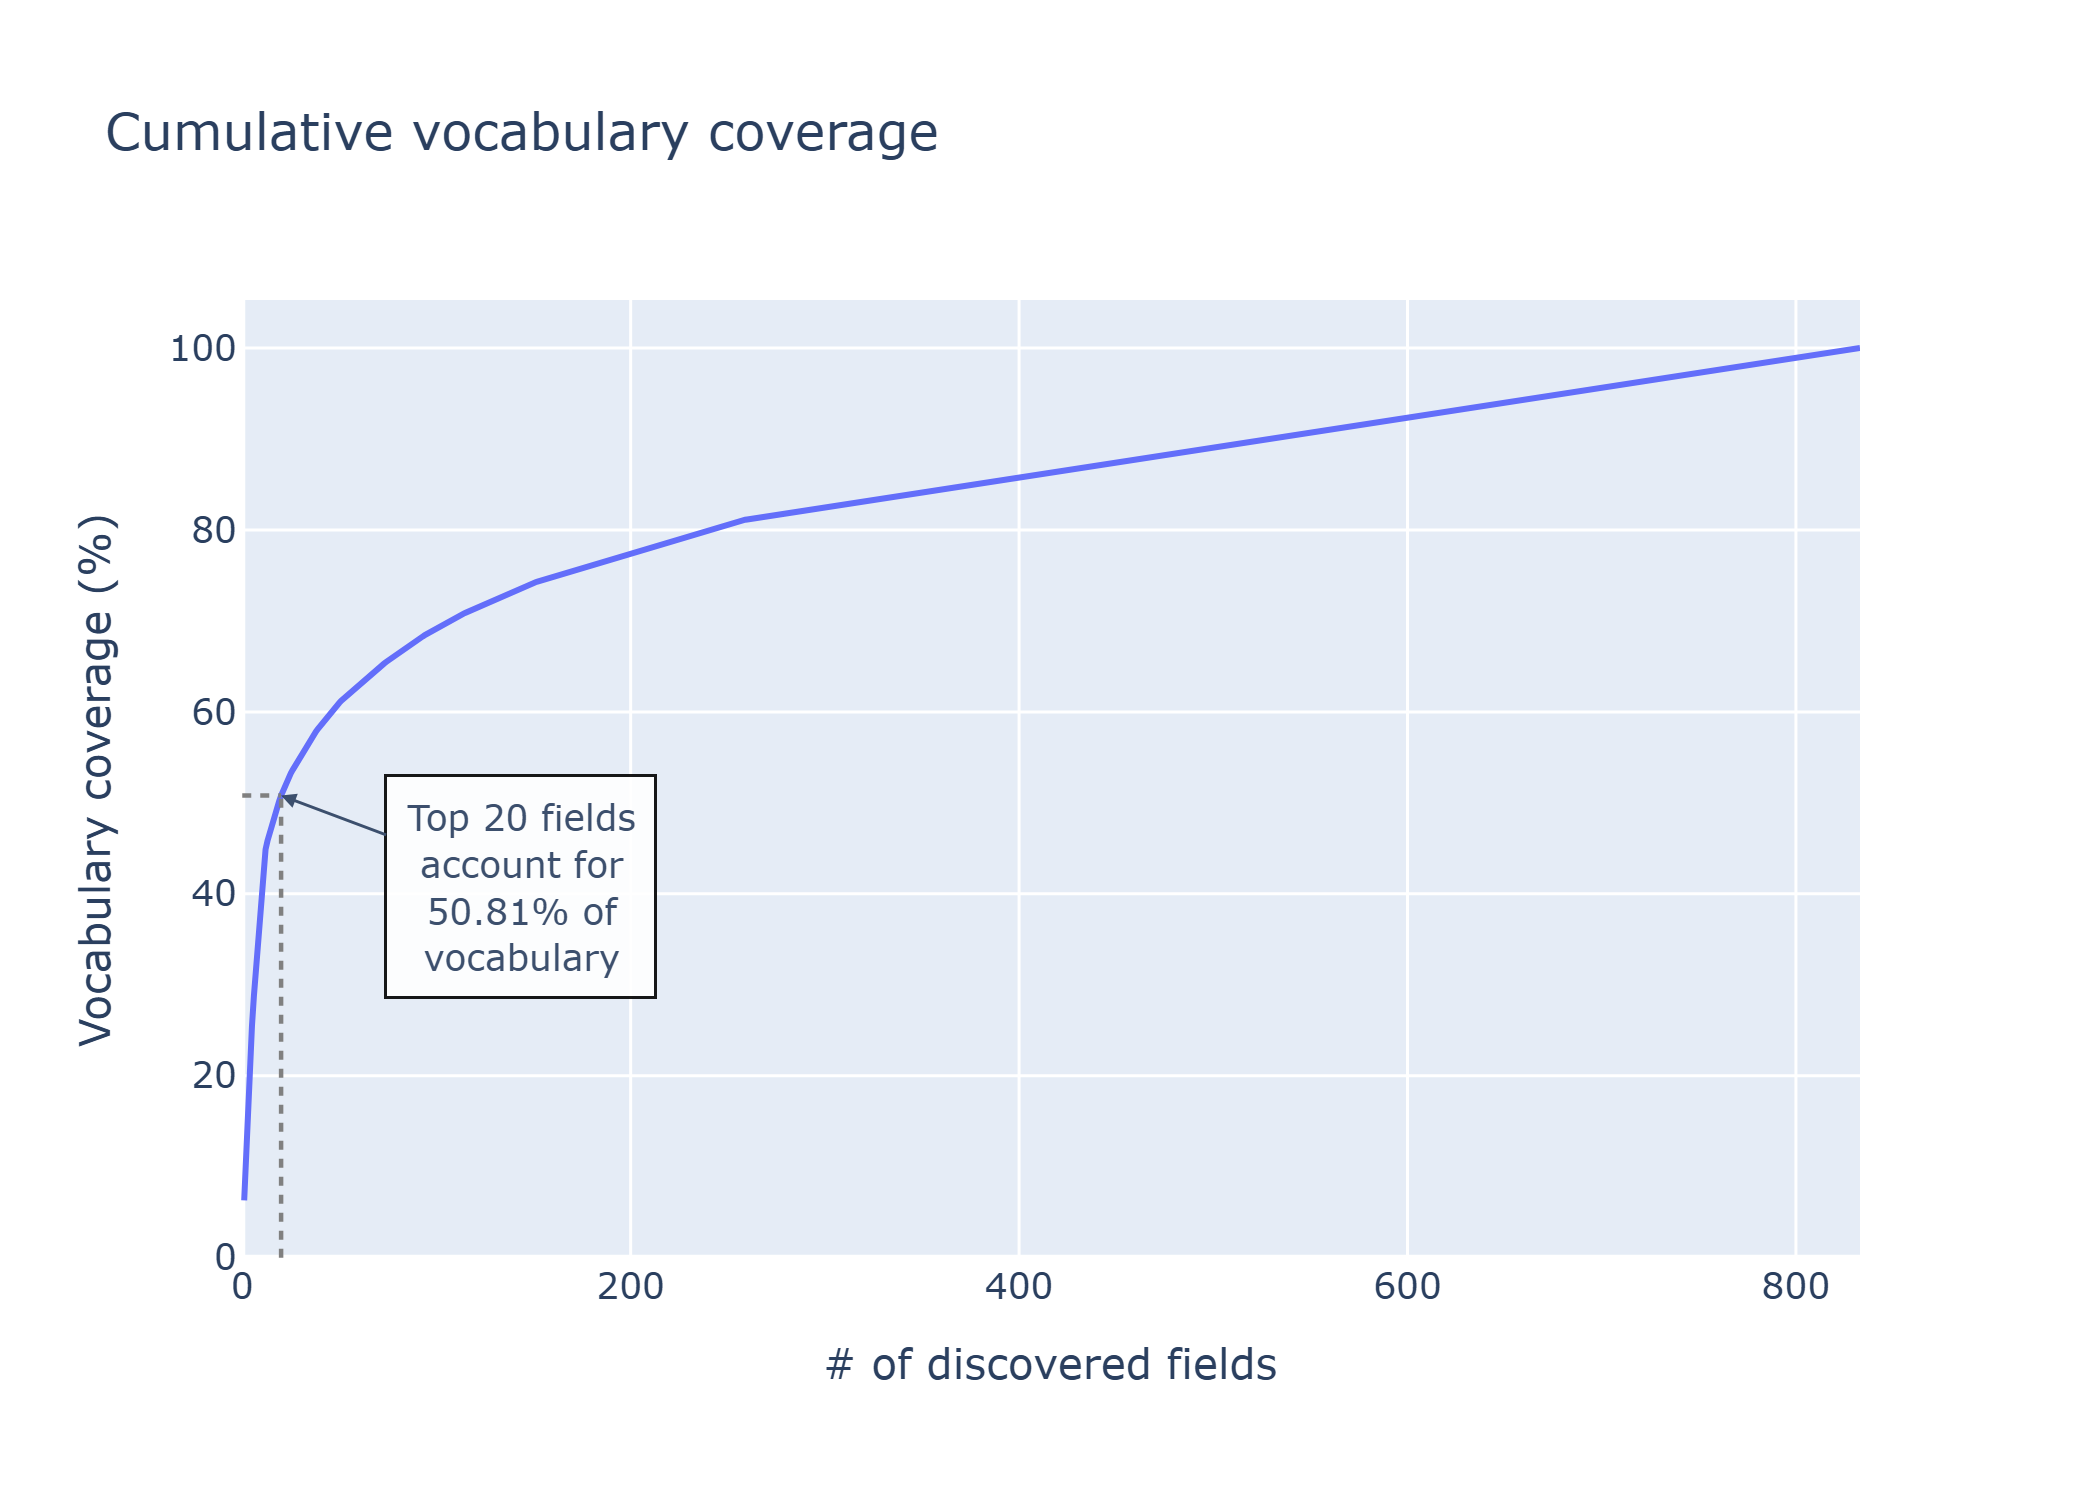
\includegraphics[width=0.75\linewidth]{data/topk_coverage.png}
\caption{Cumulative observation coverage as additional discovered metadata fields are included in descending order of frequency. The top 20 most frequently proposed metadata fields cover half of all observations. [TODO: Change the embedded title, y-axis, and callout from ``vocabulary coverage'' to ``observation coverage.'']}
\label{fig:topk_coverage}
\end{figure}

Inspection of these singleton fields revealed that much of the apparent diversity arose from lexical variation rather than fundamentally different semantics. Semantically related concepts frequently appeared under different names, levels of abstraction, or contextual interpretations, including variations in aggregation terminology, administrative boundary descriptions, and indicator naming conventions. Consequently, the long tail reflects both genuine semantic diversity and the absence of early vocabulary normalization.

The discovered vocabulary also continued to expand throughout the development collection (Figure~\ref{fig:vocabulary_growth}). Even after all 210 development snapshots had been analyzed, each additional snapshot introduced an average of approximately four previously unseen candidate metadata fields. Repeated random shuffling of the dataset produced nearly identical accumulation curves, indicating that the continued growth was not an artifact of processing order.

Within the representative sample, the discovered vocabulary continued to expand without evidence of saturation. This suggests that representative artifact collections may require substantial semantic exploration before vocabulary growth begins to stabilize.

\begin{figure}[t]
\centering
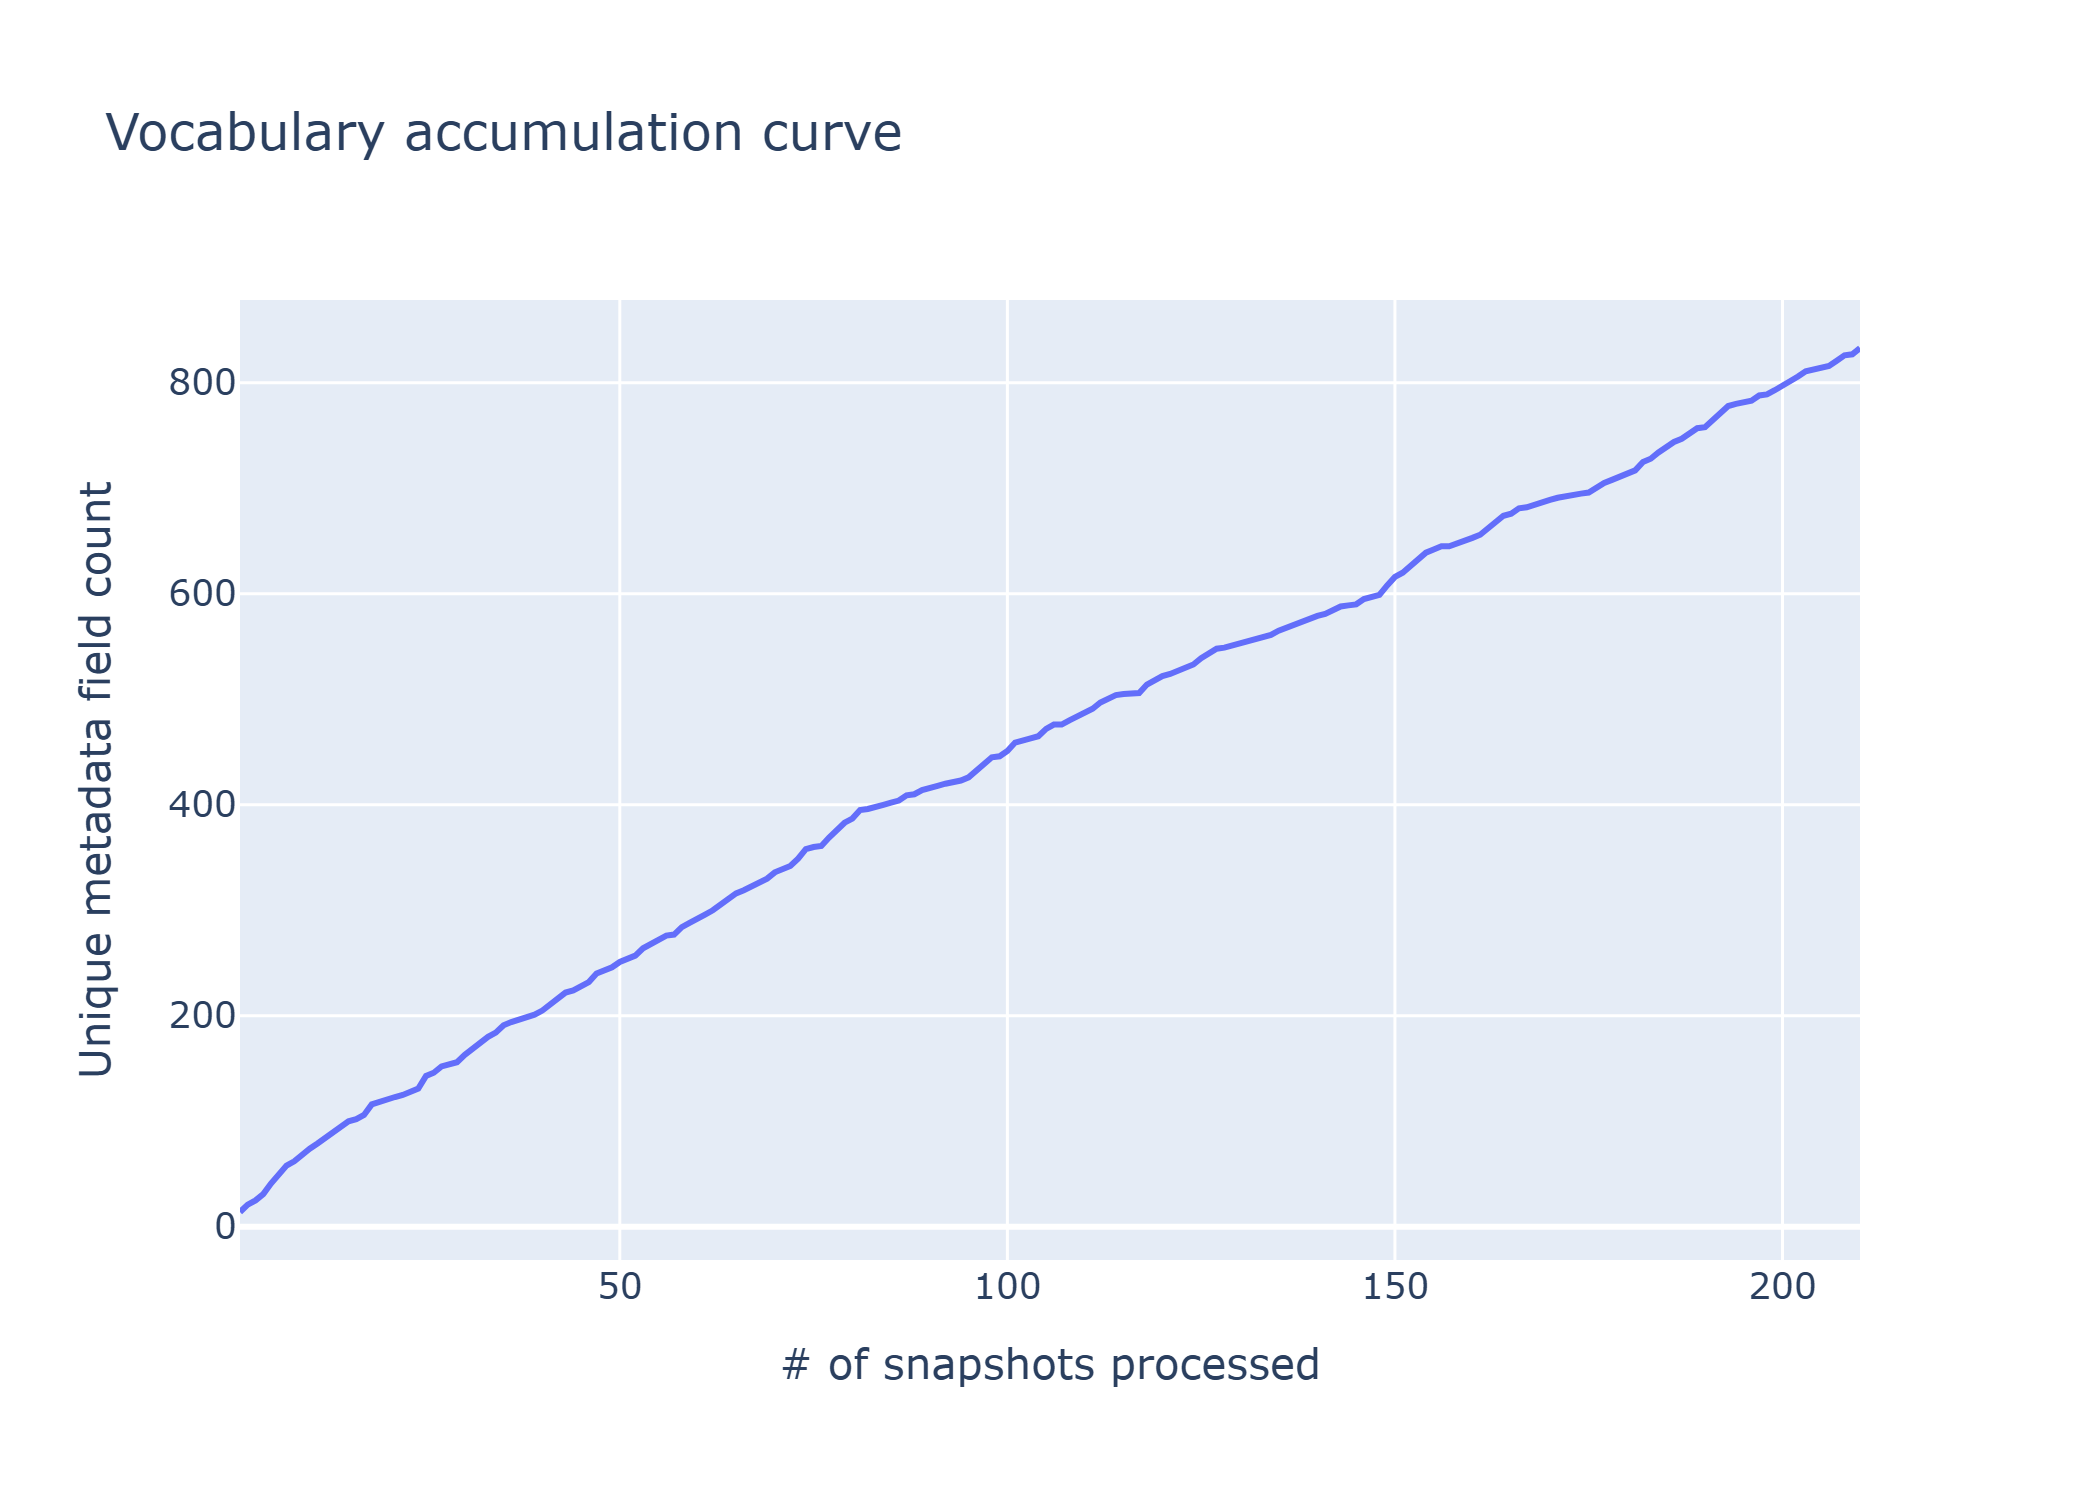
\includegraphics[width=0.75\linewidth]{data/vocabulary_growth.png}
\caption{Vocabulary accumulation curve showing the cumulative number of unique candidate metadata fields discovered as additional data snapshots were processed.}
\label{fig:vocabulary_growth}
\end{figure}

Taken together, these observations characterize independent metadata discovery as an exploratory stage of metadata schema development. Across the development collection, the process consistently identified candidate metadata while exposing a large and continually expanding vocabulary. Many discovered fields were lexical variants of related concepts, but retaining this diversity provided a broad evidential basis for subsequent concept synthesis.

\subsection{Metadata field profiles as reusable semantic evidence}

Metadata discovery produces localized observations that preserve semantic diversity but are too numerous for direct concept synthesis. Metadata field profiles bridge this gap by aggregating observations that share the same candidate field into a single evidence-bearing representation.

Aggregating the 3,041 metadata observations resulted in 833 metadata field profiles, reducing the number of semantic units requiring subsequent analysis by approximately 73\% (Table~\ref{tab:aggregation_summary}). Importantly, aggregation did not perform any semantic abstraction. Aggregation simply combined repeated occurrences of identical candidate metadata fields while preserving the supporting evidence associated with each field, including representative observed values, descriptive summaries, explanatory reasoning, and occurrence statistics.

\begin{table}[!ht]
    \centering
    \caption{Effect of metadata field profile aggregation.}
    \label{tab:aggregation_summary}
    \begin{tabular}{lr}
        Number of metadata observations & 3,041 \\
        Number of metadata field profiles & 833 \\
        Reduction & 72.6\% \\
    \end{tabular}
\end{table}

The principal effect of aggregation was not compression alone, but a change in the unit of semantic reasoning. Each metadata observation represents a localized interpretation of one artifact. A metadata field profile instead summarizes the collective evidence associated with a candidate field across the development collection. Concept synthesis therefore operates on evidence-bearing profiles rather than thousands of isolated observations.

This change enriches the evidence available for conceptual abstraction. Individual observations contain evidence from one artifact. Metadata field profiles accumulate representative values, descriptive summaries, rationales, occurrence statistics, and empirical support across multiple artifacts. Concept synthesis can therefore compare candidate fields using their accumulated semantic characteristics rather than their names alone.

\begin{table}[!ht]
    \centering
    \caption{Illustrative metadata field profile generated through aggregation. Each profile consolidates metadata observations sharing the same candidate metadata field into a reusable semantic evidence unit.}
    \label{tab:field_profile_example}
    \renewcommand{\arraystretch}{1.4}
    \newcolumntype{Y}[1]{>{\hsize=#1\hsize\raggedright\arraybackslash}X}
    \begin{tabularx}{\textwidth}{Y{0.6} Y{1.4}}
    \toprule
    
    \textbf{Metadata field profile component} & \textbf{Example content} \\
    \midrule
    
    Candidate metadata field & \texttt{geographic\_scope} \\
    
    Occurrence count & 192 metadata observations \\
    
    Representative values & Lebanon, Djibouti, Uganda, Croatia, World \\
    
    Representative descriptions &
    • Country or geographic area to which the table applies.\newline
    • Broad geographic region covered by the visualization. \\
    
    Representative reasoning &
    • Enables country-level search, filtering, and comparison.\newline
    • Provides geographic context for retrieval. \\

    Corpora represented & 3 corpora \\
    
    Artifact distribution & 96 figures, 96 tables \\

    \bottomrule
    \end{tabularx}
\end{table}

Inspection of representative field profiles (Table~\ref{tab:field_profile_example}) illustrates the value of this richer representation. Frequently occurring metadata fields accumulated diverse values, semantic descriptions, explanatory rationale, occurrence statistics, and provenance across many artifacts, while less common fields likewise retained sufficient contextual evidence for semantic interpretation.

Metadata field profiles therefore do more than reduce the number of semantic units requiring analysis. They transform localized observations into reusable semantic evidence while preserving the diversity discovered during the previous stage. This intermediate representation connects independent discovery to shared concept synthesis. Metadata field profiles emerged during implementation rather than being specified in the initial workflow design, illustrating how intermediate knowledge artifacts can clarify the reasoning required between stages.

\subsection{Progressive concept synthesis and expert refinement}

Metadata field profiles preserve rich semantic evidence but remain too numerous for direct expert review. Two complementary stages transformed the 833 profiles into a coherent metadata concept inventory: conservative LLM-assisted concept synthesis followed by iterative expert refinement. This separation assigned semantic consolidation and final conceptual decisions to distinct stages (Table~\ref{tab:ontology_progression}).

\begin{table}[!ht]
    \centering
    \caption{Progressive reduction in semantic units during concept synthesis and expert refinement.}
    \label{tab:ontology_progression}
    \begin{tabular}{lr}
    \toprule
        \textbf{Stage} & \textbf{Semantic units} \\
        \midrule
        Metadata field profiles & 833 \\
        Candidate metadata concept inventory & 70 \\
        Refined metadata concept inventory & 41 \\
    \bottomrule
    \end{tabular}
\end{table}

Canonical metadata concept synthesis consolidated the discovered semantic space by grouping metadata field profiles that represented the same underlying concept despite differences in terminology, disciplinary perspective, or level of abstraction. Rather than maximizing semantic compression, the multimodal LLM was instructed to merge conservatively and retain plausible distinctions when uncertainty remained. This reduced 833 field profiles to a candidate inventory of 70 concepts intended to apply across the reporting domains represented in the case study. The reduction made the evidence more tractable for expert review while preserving distinctions that required human adjudication. Expert refinement then transformed the candidate inventory into a refined inventory of 41 concepts through recurring decisions to merge, rename, or exclude concepts (Table~\ref{tab:ontology_decisions}).

\begin{table}[!ht]
    \centering
    \caption{Representative expert concept-refinement decisions.}
    \label{tab:ontology_decisions}
    \renewcommand{\arraystretch}{1.4}
    \newcolumntype{Y}[1]{>{\hsize=#1\hsize\RaggedRight\arraybackslash}X}
    \renewcommand{\tabularxcolumn}[1]{m{#1}}
    
    \begin{tabularx}{\textwidth}{Y{0.4} Y{1.15} Y{1.45}}
    \toprule
        \textbf{Decision} & \textbf{Representative examples} & \textbf{Rationale} \\
        \midrule
        Concept merge &
          \texttt{measure\_name} \newline \quad $\rightarrow$ \texttt{indicator\_name} \newline
          \texttt{axis\_variable} \newline \quad $\rightarrow$ \texttt{indicator\_name} \newline
          \texttt{outcome\_variable} \newline \quad $\rightarrow$ \texttt{indicator\_name} &
          These are equivalent analytical variables expressed using different visualization or disciplinary terminology. \\
        \midrule
        Concept rename &
          \texttt{presentation\_type} \newline
          \quad $\rightarrow$ \texttt{visualization\_type} &
          This improves conceptual clarity and broader applicability across visualization types. \\
        \midrule
        Concept exclusion &
          \texttt{data\_values} \newline
          \texttt{legend\_semantics} &
          These represent extracted content rather than reusable metadata concepts. \\
    \bottomrule
    \end{tabularx}
\end{table}

Separating concept synthesis from expert refinement reduced the complexity of the discovered semantic space without assigning final conceptual decisions to the LLM. Conservative synthesis retained uncertain distinctions for review. Expert refinement then resolved the remaining ambiguities without requiring direct comparison of all 833 metadata field profiles. The resulting process reduced the review space while preserving human control over the refined concept inventory.

\subsection{Empirical concept coverage assessment}
\label{sec:validation}

Following expert refinement, each metadata field profile was assigned to a concept in the refined inventory. Quantitative analyses examined concept frequency, corpus coverage, artifact-type coverage, and representative assignments, including the historical \texttt{not\_in\_ontology} output label. These analyses assessed whether the inventory contained unsupported distinctions, inappropriate boundaries, or omissions that warranted further refinement.

Concept frequencies exhibited a head--tail distribution (Table~\ref{tab:ontology_frequency}), with a small number of broadly applicable concepts and a longer tail of specialized concepts. Low empirical support alone was insufficient evidence that a concept should be merged or removed.

\begin{table}[!ht]
    \centering
    \caption{Metadata concepts with the highest and lowest snapshot support.}
    \label{tab:ontology_frequency}
    % Automatically scales the combined tables down to the text width
    \resizebox{\textwidth}{!}{
        \begin{tabular}{lrr}
        \toprule
        \multicolumn{3}{c}{\textbf{Highest support}} \\
        \midrule
        \textbf{Concept} & \textbf{Count} & \textbf{Support} \\
        \midrule
        \texttt{title} & 195 & 92.9\% \\
        \texttt{indicator\_name} & 194 & 92.4\% \\
        \texttt{geographic\_scope} & 194 & 92.4\% \\
        \texttt{unit\_of\_measure} & 185 & 88.1\% \\
        \texttt{time\_period} & 156 & 74.3\% \\
        \bottomrule
        \end{tabular}
        \quad
        \begin{tabular}{lrr}
        \toprule
        \multicolumn{3}{c}{\textbf{Lowest support}} \\
        \midrule
        \textbf{Concept} & \textbf{Count} & \textbf{Support} \\
        \midrule
        \texttt{indicator\_definition} & 11 & 5.2\% \\
        \texttt{financing\_source} & 10 & 4.8\% \\
        \texttt{data\_collection\_method} & 9 & 4.3\% \\
        \texttt{project\_component} & 8 & 3.8\% \\
        \texttt{financing\_instrument} & 7 & 3.3\% \\
        \bottomrule
        \end{tabular}
    }
\end{table}

Inspection of assignments to lower-support concepts showed that they represented legitimate domain-specific metadata rather than redundant concepts (Table~\ref{tab:ontology_validation}). Field profiles assigned to \texttt{not\_in\_ontology} predominantly contained analytical values and other intentionally excluded content rather than missing metadata concepts. The historical label is retained here because it appears in the case-study output.

\begin{table}[!ht]
    \caption{Representative concept coverage observations for low-support and excluded concepts.}
    \label{tab:ontology_validation}
    \renewcommand{\arraystretch}{1.4}
    \renewcommand{\arraystretch}{1.4}
    \newcolumntype{Y}[1]{>{\hsize=#1\hsize\RaggedRight\arraybackslash}X}
    \renewcommand{\tabularxcolumn}[1]{m{#1}}

    \begin{tabularx}{\textwidth}{Y{0.8} Y{1.1} Y{1.1}}
    \toprule
        \textbf{Validation observation} &
    \textbf{Representative examples} &
    \textbf{Interpretation} \\
    
    \midrule
    
    Specialized metadata concepts &
    \texttt{project\_component} \newline
    \texttt{financing\_source} \newline
    \texttt{data\_collection\_method} &
    These concepts occurred infrequently because they were associated with specialized document collections or analytical contexts rather than representing redundant concepts. \\
    
    \midrule
    
    \texttt{not\_in\_ontology} assignments &
    \texttt{sample\_size} \newline
    \texttt{measure\_values} \newline
    \texttt{axis\_range} \newline
    \texttt{summary\_total} &
    These assignments predominantly represented analytical values and quantitative content intentionally excluded from the metadata concept inventory, confirming the intended boundary between metadata and extracted content. \\
    \bottomrule
    \end{tabularx}
\end{table}

Overall, the assessment found no compelling evidence that the refined inventory required further conceptual revision before schema design. It provided an empirical characterization of the inventory and a basis for reviewing low-support and excluded concepts.

\subsection{Operational metadata schema design}

The refined inventory provided the conceptual foundation for metadata schema design, which transformed 41 concepts into the Data Snapshot Metadata Schema with 36 fields. The objective shifted from establishing conceptual distinctions to representing those distinctions for consistent annotation and retrieval.

\begin{table}[!ht]
    \centering
    \caption{Representative metadata schema design decisions.}
    \label{tab:schema_decisions}
    \renewcommand{\arraystretch}{1.4}
    \newcolumntype{Y}[1]{>{\hsize=#1\hsize\RaggedRight\arraybackslash}X}
    \renewcommand{\tabularxcolumn}[1]{m{#1}}
    \begin{tabularx}{\textwidth}{Y{0.4} Y{1.1} Y{1.5}}
    \toprule
    
    \textbf{Decision} &
    \textbf{Representative example} &
    \textbf{Operational rationale} \\
    \midrule
    
    Merge &
    \texttt{series\_labels} \newline \quad $\rightarrow$ \texttt{indicator\_name} 
    \newline
    \texttt{calculation\_method} \newline \quad $\rightarrow$ \texttt{analysis\_method}
    &
    Unified semantically related concepts within a snapshot without reducing practical expressiveness. \\
    
    \midrule
    
    Reintroduce &
    \texttt{panel\_title} &
    Support annotation of multi-panel figures. \\
    
    \midrule
    
    Remove &
    \texttt{indicator\_definition} &
    Excluded concepts whose operational value did not justify maintaining an independent metadata field. \\
    
    \midrule
    
    Rename &
    \texttt{financial\_metric} \newline \quad $\rightarrow$ \texttt{financial\_measure} &
    Improved terminology clarity and consistency throughout the deployed schema. \\
    
    \midrule
    
    Refine &
    \texttt{comparison\_group} \newline
    \texttt{reference\_date} &
    Broadened or clarified concept definitions to improve applicability across diverse document collections. \\
    
    \bottomrule
    \end{tabularx}
\end{table}

Representative decisions are summarized in Table~\ref{tab:schema_decisions}. These decisions were guided by operational considerations in addition to semantic distinctiveness. Concepts were merged when separate fields offered little practical benefit, reintroduced when operational requirements justified restoring a distinction, renamed or refined to improve clarity and applicability, or removed when their value did not justify additional annotation complexity.

Schema design also reintroduced concepts when operational requirements justified restoring distinctions removed during concept refinement. For example, \texttt{panel\_title} had been merged into \texttt{title} because the distinction was not considered necessary in the concept inventory. It was reinstated as an independent field to support annotation and retrieval of multi-panel figures. The operational schema therefore does not reproduce the refined inventory one-to-one.

The resulting fields were organized into nine semantic modules representing complementary aspects of data snapshot metadata. These modules support readability and annotation guidance; they organize the specification without asserting a conceptual hierarchy.

Metadata schema design completed the transition from a refined concept inventory to an operational specification. The reduction from 41 concepts to 36 fields reflects operational representation decisions rather than a loss of traceability to the underlying concept evidence.

\subsection{Held-out schema validation}

The two validation exercises examined whether the operational schema remained adequate when applied beyond the 210-snapshot development collection (Table~\ref{tab:schema_validation_results}). Validation 1 retained an open discovery mode and produced 578 candidate-field proposals. Human adjudication showed that semantic difference alone did not justify a field: many proposals described parent documents, analytical values, specialized details, or structural relationships rather than missing top-level snapshot metadata.

The documentation-only revision following Validation 1 records an additional function of validation. Evaluation may reveal ambiguity in field definitions or scope even when it does not justify changing the field inventory. Schema validation can therefore produce documentation changes, representation requirements, or confirmed exclusions in addition to new fields.

Validation 2 narrowed the assessment to omissions with material consequences for interpretation or discovery. This reduced the positive review set to six possible gaps across five snapshots. Human adjudication again accepted no new field and classified two candidates as representation limitations. The result distinguishes vocabulary coverage from representational adequacy: an existing concept may be present while a flat schema remains unable to preserve relationships among panels, variables, or hierarchical table structures.

Together, the exercises provide evidence that the 36-field inventory was stable with respect to the tested held-out collection and intended application. This conclusion concerns the accepted inventory after human review. It does not imply that candidate generation had saturated or that the schema will cover every future artifact without ambiguity.

Viewed collectively, the six transformations show that metadata schema development is not a single inference task. Each intermediate knowledge artifact reduces or reorganizes semantic complexity while preserving evidence for the next stage. Held-out validation then tests the operational result and returns candidate gaps to human review. This structure assigns artifact interpretation and large-scale semantic comparison to LLM-supported stages while preserving human responsibility for conceptual boundaries, operational design, and schema revision.

\section{Discussion}

\subsection{Artifact-driven metadata schema development}

The case study illustrates how established principles from metadata profile development, schema discovery, ontology learning, and multimodal document understanding can be adapted to derive a metadata schema from the artifacts it must describe. The central design choice is to delay construction of a shared vocabulary until each artifact has been analyzed independently. This preserves local observations that might otherwise be absorbed prematurely into concepts established from earlier artifacts.

Metadata field profiles then aggregate these observations without removing their descriptions, examples, occurrence patterns, or provenance. The resulting evidence-bearing representation supports concept synthesis across artifacts while retaining a path back to the observations that motivated each concept. The candidate and refined metadata concept inventories further reduce the review space, but they do not determine the operational schema directly. Schema design introduces a separate set of decisions concerning field organization, annotation guidance, representational simplicity, and intended use. The difference between the 41 concepts in the refined inventory and the 36 fields in the Data Snapshot Metadata Schema reflects this change in objective.

This sequence distinguishes conceptual consolidation from operational representation. A concept may remain distinct because it captures a meaningful descriptive requirement, yet be combined with another concept in the schema when a separate field offers limited practical value. Conversely, a distinction removed during concept refinement may be restored when it supports annotation or retrieval, as occurred with \texttt{panel\_title}. The schema is therefore an operationalization of the concept inventory rather than a direct encoding of it.

The intermediate knowledge artifacts also make the development process inspectable. Schema fields can be related to refined concepts, field profiles, and artifact-level observations, enabling reviewers to examine both the resulting decision and its supporting evidence. This traceability does not eliminate expert judgment, but it makes the basis for revision more explicit than a workflow that produces the schema in a single inference step.

\subsection{Human--LLM collaboration across semantic transformations}

The case study supports a division of responsibility in which multimodal LLMs perform bounded semantic tasks and human experts retain authority over conceptual and operational decisions. The LLM interpreted individual artifacts, synthesized related evidence into candidate concepts, and performed constrained classification during concept coverage assessment and schema validation. Deterministic aggregation connected artifact-level observations to reusable field profiles without additional model inference.

Human review governed the decisions for which semantic similarity was insufficient. These included defining the boundary between metadata and analytical content, deciding whether concepts should be merged or retained, determining whether a concept warranted an independent field, and adjudicating proposed schema gaps. Such decisions depend on the intended scope and use of the metadata schema. They cannot be resolved solely from linguistic or visual similarity among observations.

The contribution of the intermediate artifacts is therefore not automation of schema design, but reorganization of the expert task. Independent observations expose the breadth of the descriptive space; field profiles assemble evidence across artifacts; candidate concepts reduce the number of units requiring comparison; and validation outputs focus review on possible gaps. The case study shows that this arrangement can support one complete development process. It does not establish that the workflow is faster or more reliable than expert-only or alternative human--AI approaches, which were not evaluated here.

\subsection{Schema validation as part of development}

The two validation exercises show why schema validation is better treated as part of iterative development than as a final test that produces a binary verdict. Validation 1 generated 578 candidate-field proposals, but human review accepted none as a new field. The proposals nevertheless identified ambiguous definitions, scope questions, and limitations of the flat representation. The resulting documentation revision was therefore a substantive validation outcome even though the field inventory remained unchanged.

Validation 2 applied a narrower materiality criterion and produced six possible gaps across five snapshots. Human adjudication again accepted no new field, while two candidates identified representation limitations involving composite figures and hierarchical tables. These findings distinguish three questions that can otherwise be conflated: whether the schema contains the necessary metadata concept, whether its documentation defines that concept adequately, and whether its structure can preserve the required relationships. Adding a field addresses only the first of these problems.

Together, the exercises provide bounded evidence that the accepted 36-field inventory covered the metadata requirements identified in the tested collections for the intended scope. Because both exercises used the same 202 held-out snapshots, they constitute complementary assessments rather than independent replications. The absence of accepted new fields does not establish universal coverage, candidate saturation, or adequacy for artifact classes and applications outside the study.

\subsection{Broader implications and future directions}

The methodology may be useful when a class of multimodal artifacts lacks a directly adoptable metadata schema and its descriptive requirements must be established from representative artifacts. Its applicability depends on the availability and coverage of those artifacts, the multimodal model's ability to interpret them, and expert knowledge sufficient to adjudicate conceptual boundaries and operational requirements. These dependencies make transfer to other domains an empirical question rather than an assumed property of the workflow.

Future work should apply the methodology to substantially different artifact classes, compare it with expert-only and alternative human--AI workflows, and examine agreement among multiple experts during concept refinement and gap adjudication. Further work could also evaluate decision-support mechanisms for larger concept inventories and structured representations for relationships that cannot be expressed adequately through a flat field inventory.

The broader methodological implication is that metadata schema development can be organized as a sequence of evidence-preserving semantic transformations. In this formulation, multimodal LLMs support artifact interpretation and semantic comparison, deterministic procedures preserve and aggregate evidence, and human experts determine conceptual scope and operational form. The Data Snapshot Metadata Schema provides one complete case through which to examine this architecture.

\section{Limitations}

The evidence in this paper comes from one case study involving data snapshots extracted from three institutional document corpora. The 210 case study snapshots and 202 held-out snapshots cover figures and tables across different reporting contexts, but neither collection is statistically representative of institutional documents or multimodal artifacts more broadly. The resulting field inventory may reflect concepts that were present, absent, or unevenly represented in these collections. Its stability is therefore established only with respect to the tested artifacts and intended schema scope.

The two schema-validation exercises used the same 202 held-out snapshots. They provide complementary assessments of residual candidates and material omissions, but not independent replications. Validation 2 also did not include an independent human audit of every snapshot assessed as having no critical gap. The study therefore cannot estimate false-negative rates, establish candidate saturation, or rule out additional fields that may be required by future data snapshots. The resulting schema should be understood as an initial version and a starting point for continued revision as new artifacts, application requirements, and expert feedback provide additional evidence.

The methodology retains substantial dependence on expert judgment. Human decisions determined conceptual boundaries, concept merges and exclusions, operational field design, and the adjudication of proposed gaps. These decisions were made within a single case-study process rather than evaluated through multiple independent experts. The paper consequently does not establish inter-reviewer consistency or show how differences in domain expertise would affect the resulting concept inventory and schema.

The study also does not compare the methodology with expert-only development, fully automated alternatives, or other human--AI workflows. It does not measure time savings, scalability, or relative schema quality, and it does not evaluate robustness across different multimodal models, prompts, or repeated runs. The results support methodological feasibility for the reported execution rather than comparative effectiveness or model-independent reproducibility.

Finally, the operational schema remains a flat field inventory. The validation exercises identified relationships within composite figures and hierarchical tables that this representation cannot preserve fully. The paper does not evaluate subsequent technical implementation, standards alignment, interoperability, metadata-extraction accuracy, downstream retrieval performance, or community governance. These activities may require further changes to the representation, but they fall outside the methodology and evidence reported here.

\section{Conclusion}

This paper presented an artifact-driven, human-in-the-loop methodology for developing an operational metadata schema when the descriptive requirements must first be established from multimodal artifacts. The methodology organizes this process into independent metadata discovery, field profile aggregation, canonical metadata concept synthesis, expert concept refinement, concept coverage assessment, metadata schema design and specification, and held-out schema validation. Explicit intermediate knowledge artifacts preserve evidence across these semantic transformations.

The case study applied the methodology to 210 data snapshots and produced the Data Snapshot Metadata Schema with 36 fields. Two subsequent validation exercises evaluated the schema against the same 202 held-out snapshots. Human adjudication accepted no additional field, while identifying documentation ambiguities and representation limitations. These results support the feasibility of one complete execution and the stability of the accepted field inventory for the tested collections and intended scope. They do not establish universal coverage or generality beyond this case.

The workflow assigns artifact interpretation, semantic synthesis, and constrained comparison to multimodal LLMs; aggregates evidence deterministically where possible; and retains human responsibility for conceptual boundaries, operational representation, and schema revision. This division makes the transformation from visual evidence to metadata fields inspectable without treating the LLM as an autonomous schema designer.

The methodological contribution is the adaptation and integration of established principles from schema discovery, ontology learning, metadata profile development, and multimodal document understanding into an evidence-preserving sequence from artifact-level observations to an operational metadata schema. The Data Snapshot Metadata Schema provides a case through which this architecture is examined; evaluating its transfer to other artifact classes and development settings remains future work.

\subsubsection*{Acknowledgments}
This work is supported by the “Artificial intelligence for understanding data use and enhancing knowledge discovery” project funded by the World Bank-UNHC Joint Data Center on Forced Displacement - RA-P503405-RESE-TF0C7575.

\subsubsection*{Disclaimer and disclosure of AI use} 
The findings, interpretations, and conclusions expressed in this paper are entirely those of the authors. They do not necessarily represent the views of the International Bank for Reconstruction and Development/World Bank and its affiliated organizations, or those of the Executive Directors of the World Bank or the governments they represent.

This work used AI tools at various stages, including open source AI models for layout detection. In addition, NotebookLM and ChatGPT were employed to enhance the manuscript’s readability. We also thank Rafael Sevilla Macalaba for providing technical advice and suggestions to strengthen the implementation and manuscript.

\bibliographystyle{iclr2026_conference}
\bibliography{references}

\newpage

\appendix

\section{Appendix: Representative data snapshots}
\label{appendix:datasnapshots}

This appendix presents representative examples of the data snapshots used throughout the case study. The examples illustrate the diversity of analytical artifacts encompassed by the term \emph{data snapshot}, including statistical charts, tables, geospatial visualizations, dashboards, and composite analytical figures extracted from institutional PDF documents.

The examples are grouped by source corpus. Together they illustrate the range of visualization types, reporting styles, and analytical content encountered during metadata discovery and concept refinement.

\subsection{UNHCR / ReliefWeb}

Figure~\ref{fig:appendix_unhcr_dashboard} illustrates a representative composite analytical dashboard extracted from the UNHCR / ReliefWeb corpus. The snapshot integrates multiple analytical components—including key performance indicators, bar charts, flow diagrams, a geospatial map, and summary statistics—into a single information object, illustrating the heterogeneous visual and semantic content that the proposed metadata schema is intended to describe.

\begin{figure}[!ht]
    \centering
    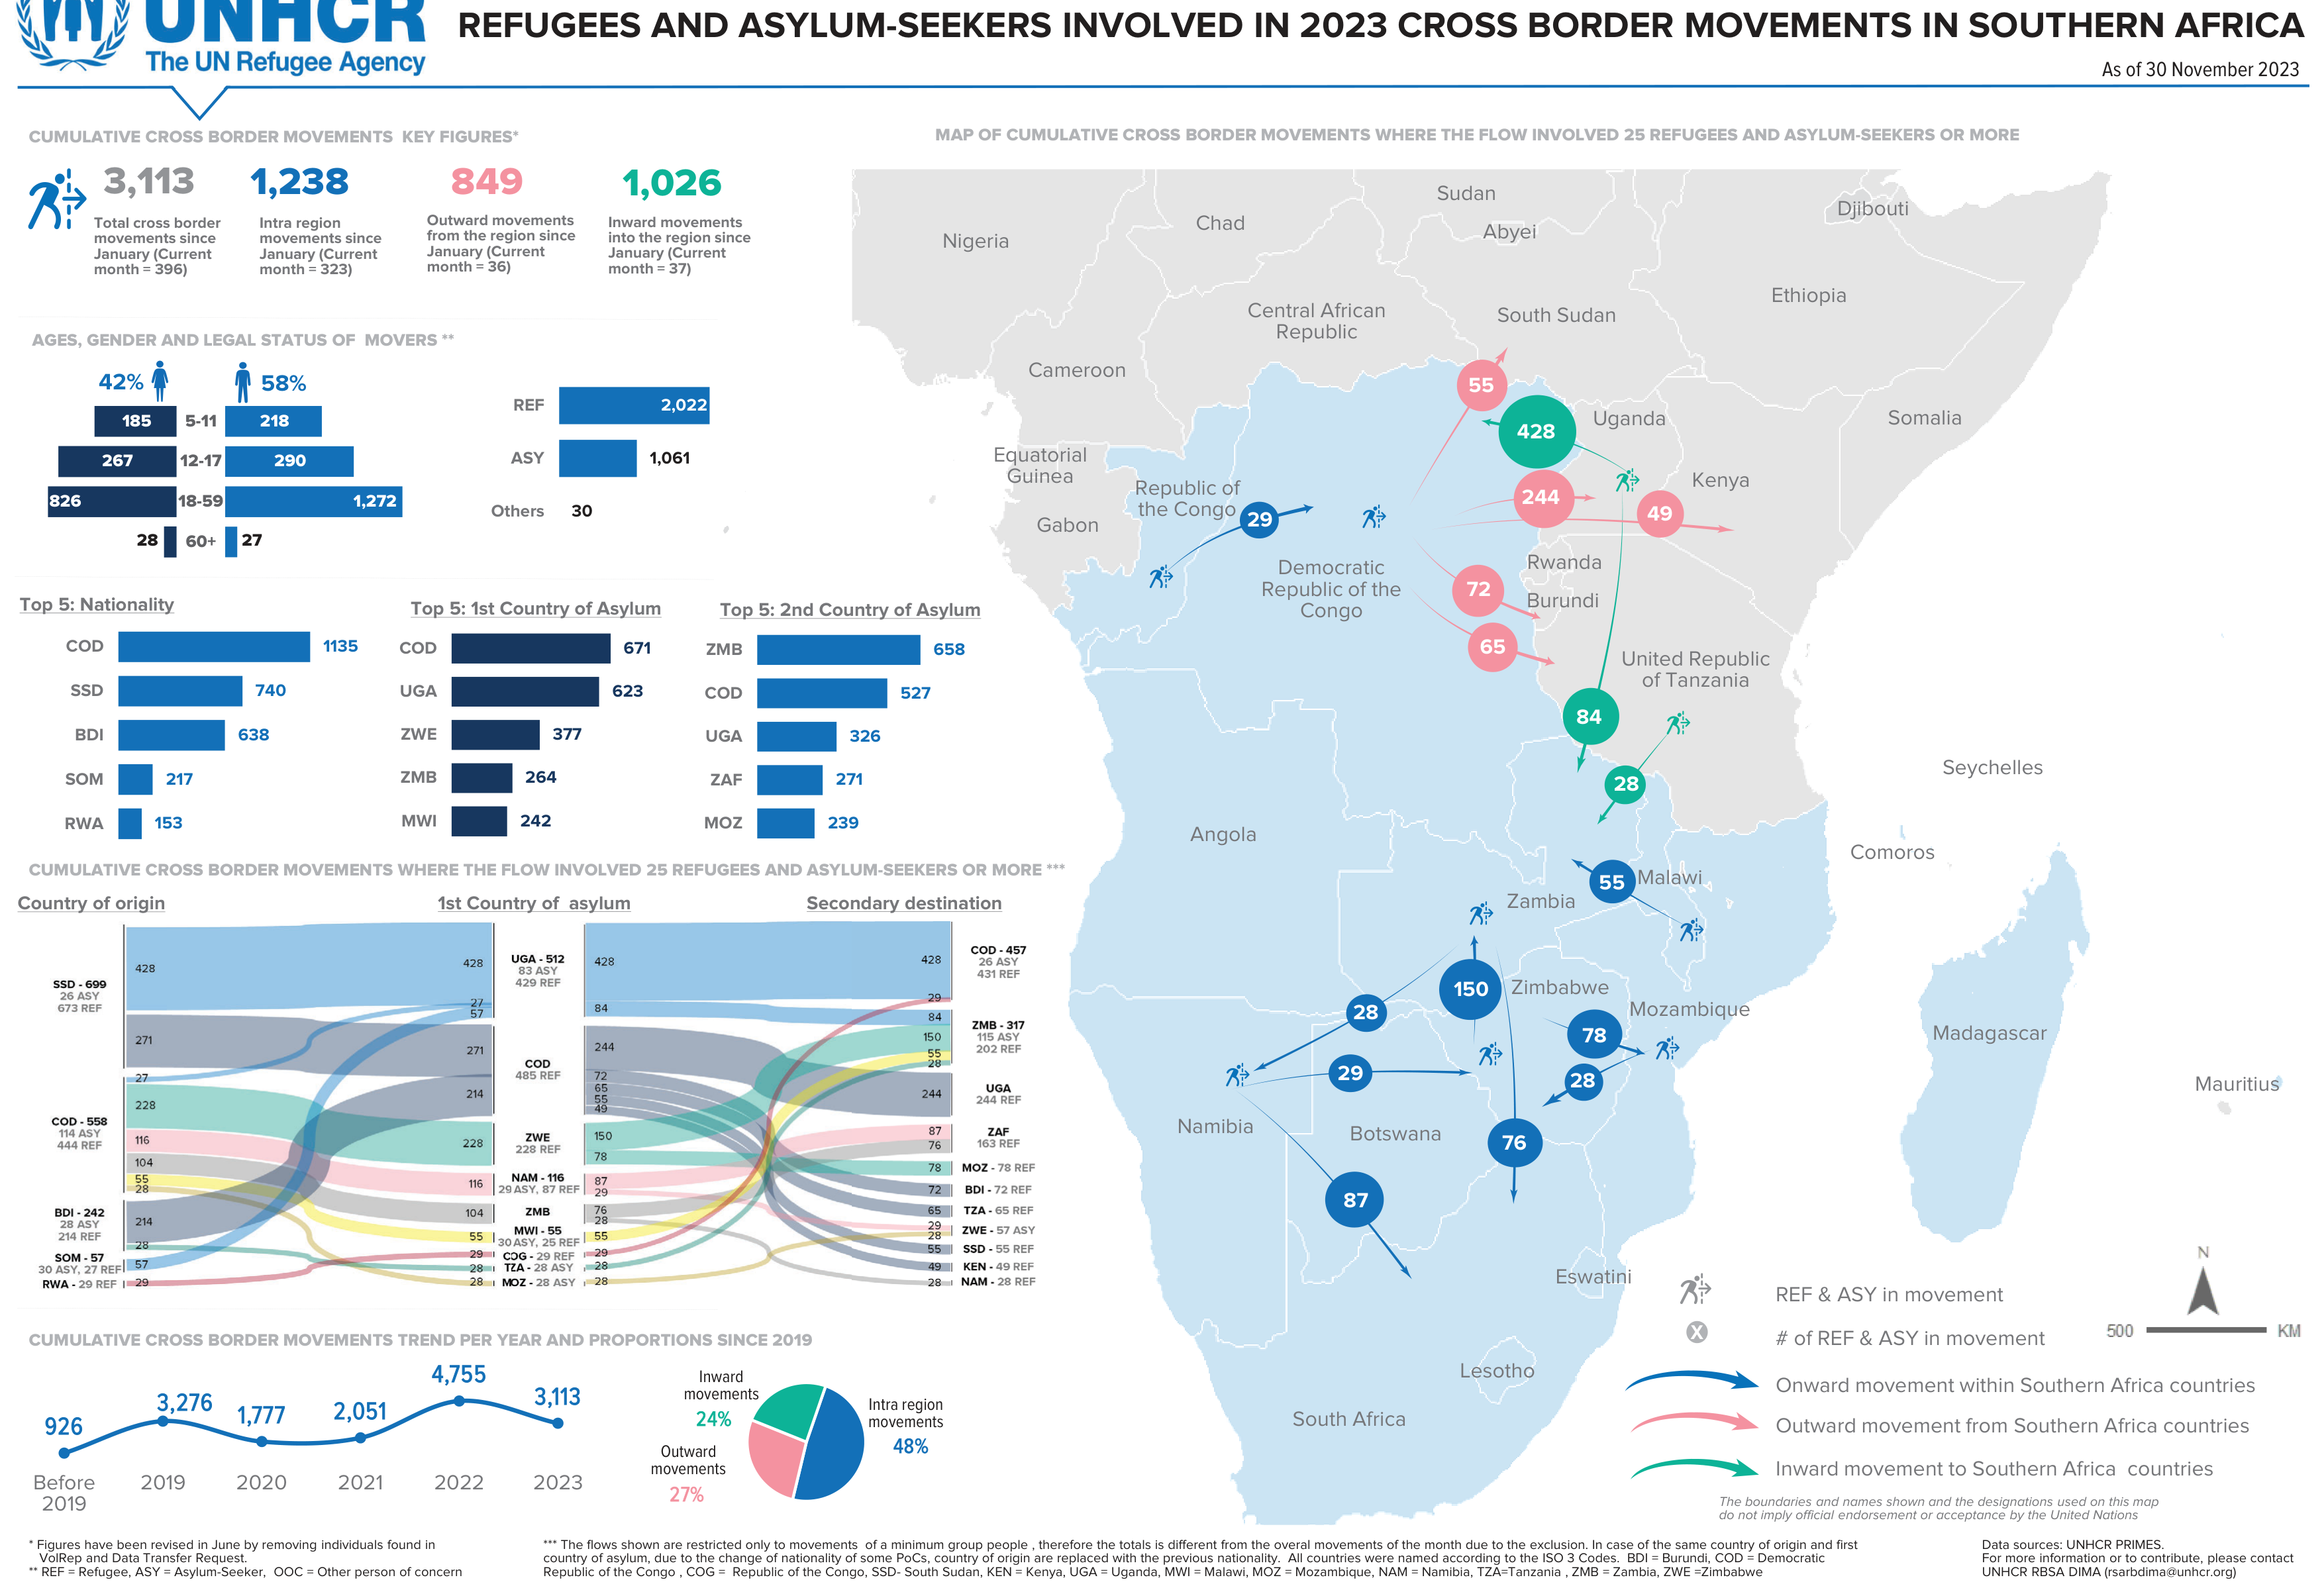
\includegraphics[width=\textwidth]{data/snapshots/nov_2023_rbsa_population_data_analysis_figure_002.png}
    \caption{Representative composite analytical dashboard from the UNHCR / ReliefWeb corpus. The snapshot combines multiple visualization types and analytical components within a single data snapshot.}
    \label{fig:appendix_unhcr_dashboard}
\end{figure}

Figure~\ref{fig:appendix_unhcr_table} presents a representative statistical table extracted from the same corpus. Together with the preceding example, it illustrates the diversity of analytical artifact types treated as data snapshots in this work.

\begin{figure}[!ht]
    \centering
    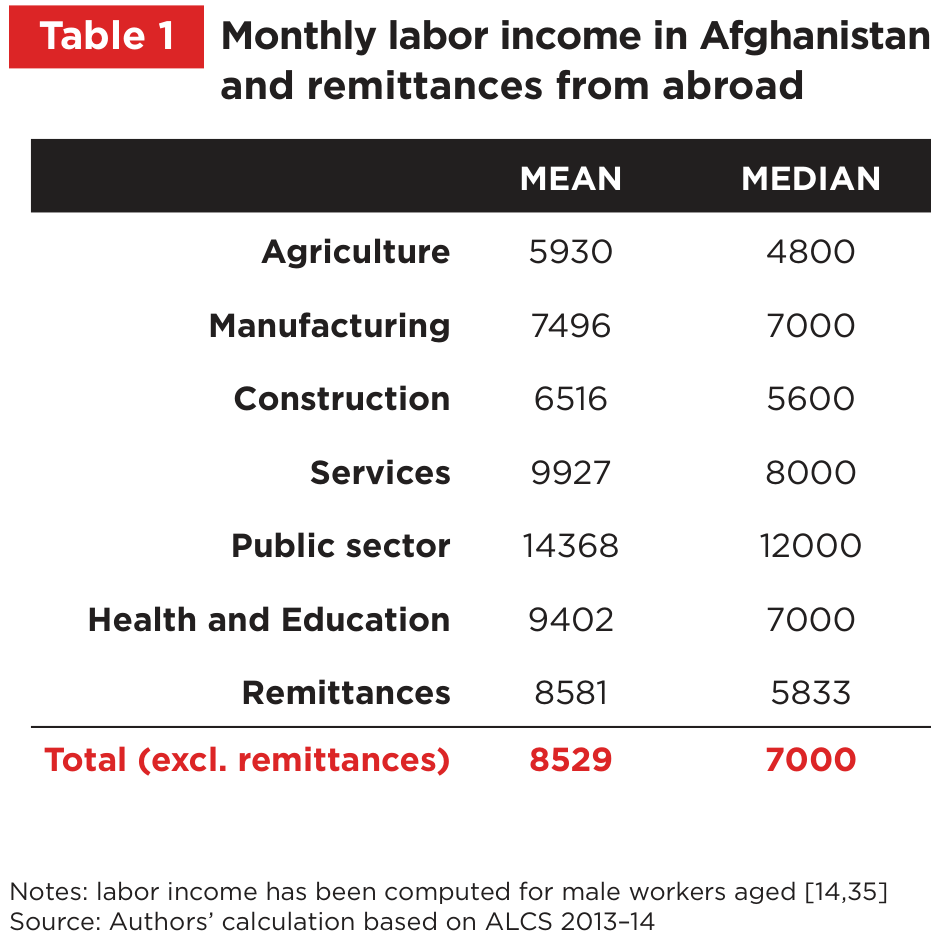
\includegraphics[width=0.5\textwidth]{data/snapshots/108733-revised-public-wb-unhcr-policy-brief-final_table_000.png}
    \caption{Representative statistical table from the UNHCR / ReliefWeb corpus illustrating a structured tabular data snapshot.}
    \label{fig:appendix_unhcr_table}
\end{figure}

\subsection{Policy Research Working Papers}

Figure~\ref{fig:appendix_prwp_map} presents a representative geospatial analytical visualization extracted from the Policy Research Working Papers corpus. The example illustrates that data snapshots include thematic maps alongside charts, tables, and other forms of analytical visualization.

\begin{figure}[!ht]
    \centering
    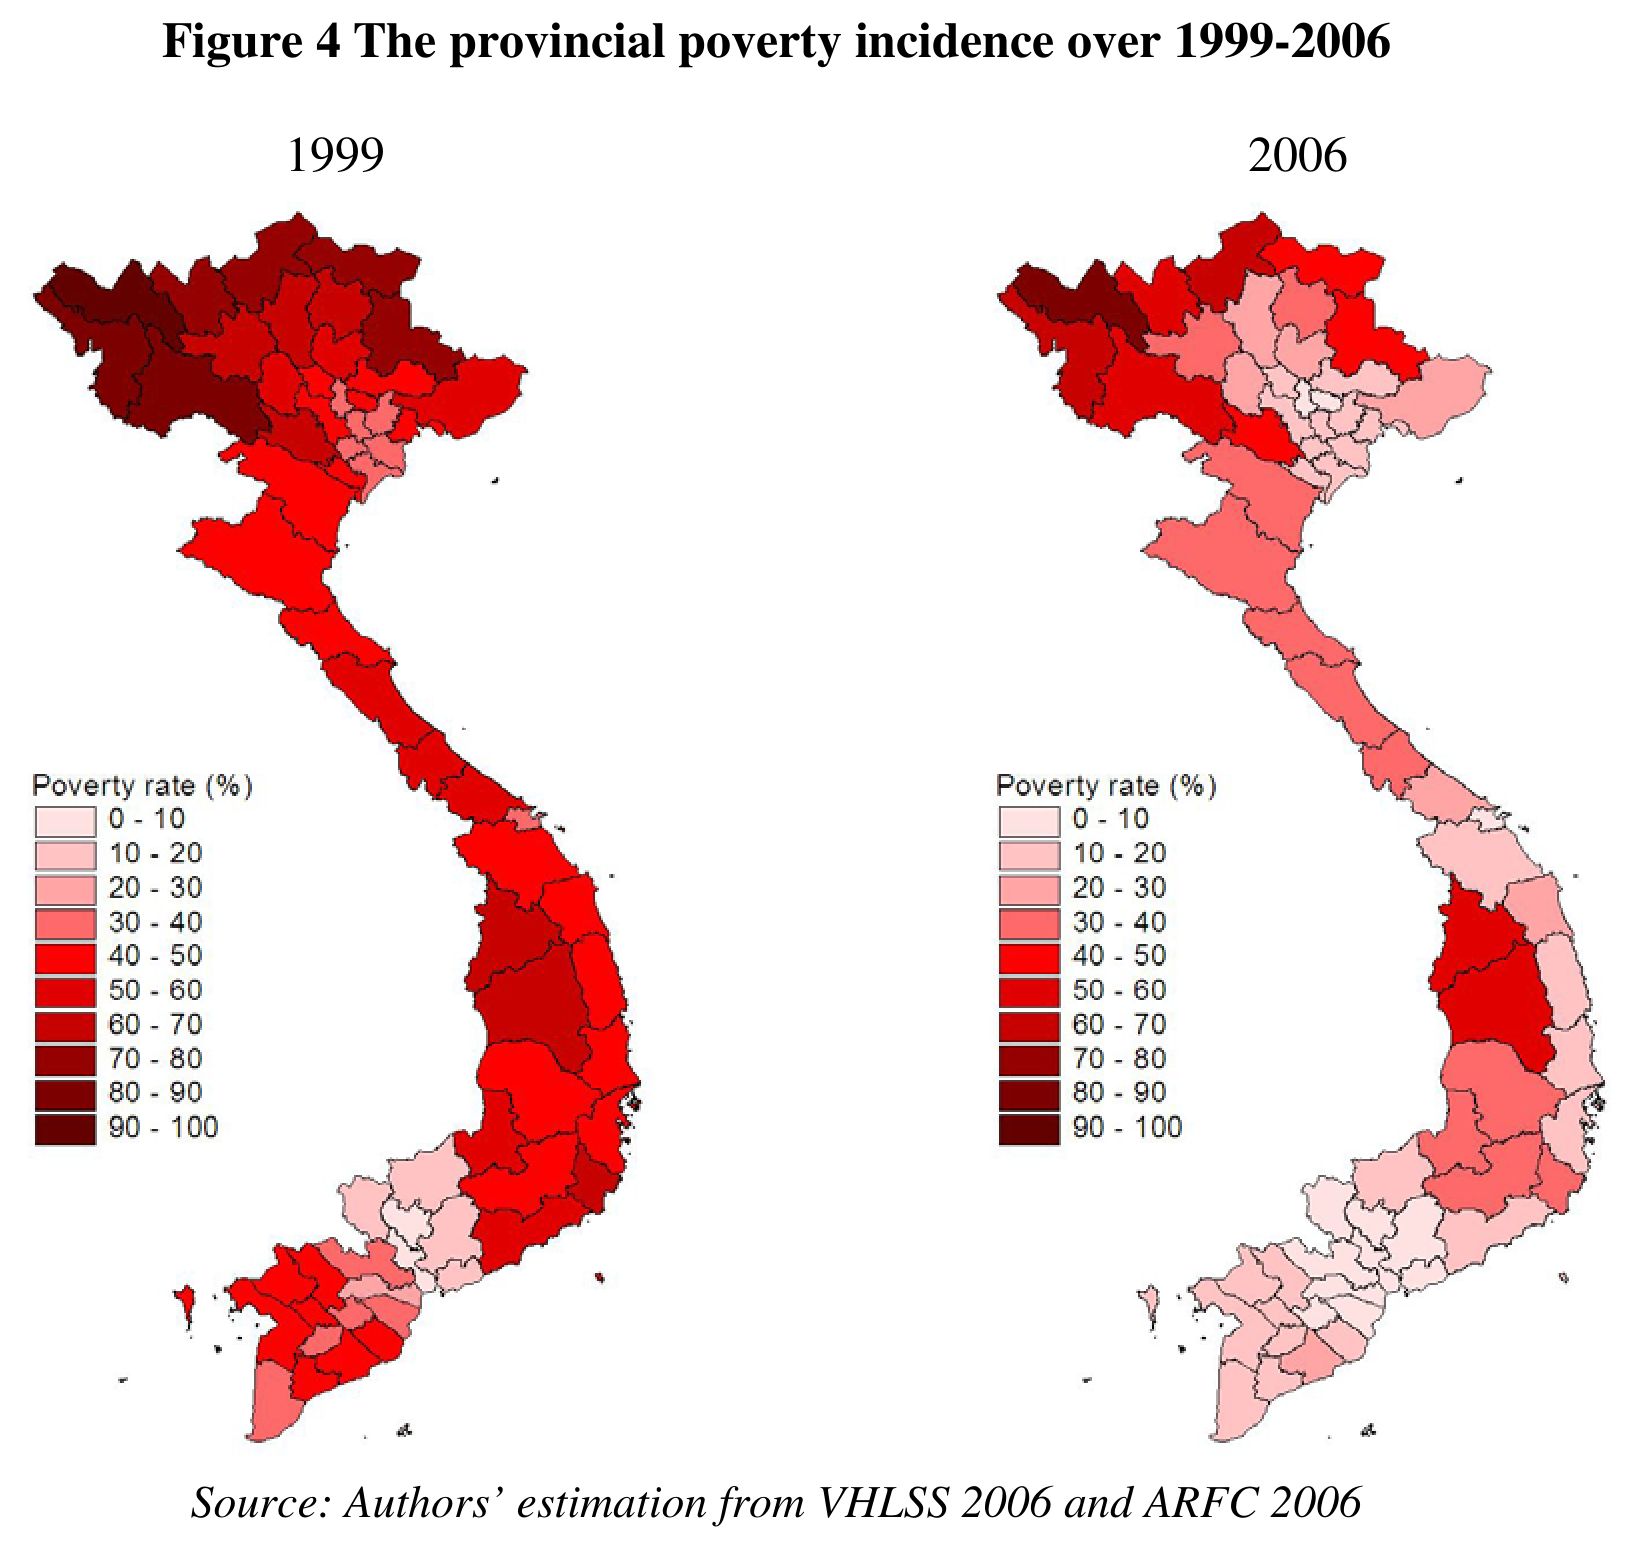
\includegraphics[width=0.5\textwidth]{data/snapshots/document_13148967_figure_003.png}
    \caption{Representative geospatial analytical visualization from the Policy Research Working Papers corpus.}
    \label{fig:appendix_prwp_map}
\end{figure}

Figure~\ref{fig:appendix_prwp_table} presents a representative statistical table extracted from the Policy Research Working Papers corpus. The example illustrates the structured tabular presentation of variables and quantitative information commonly found in academic policy research.

\begin{figure}[!ht]
    \centering
    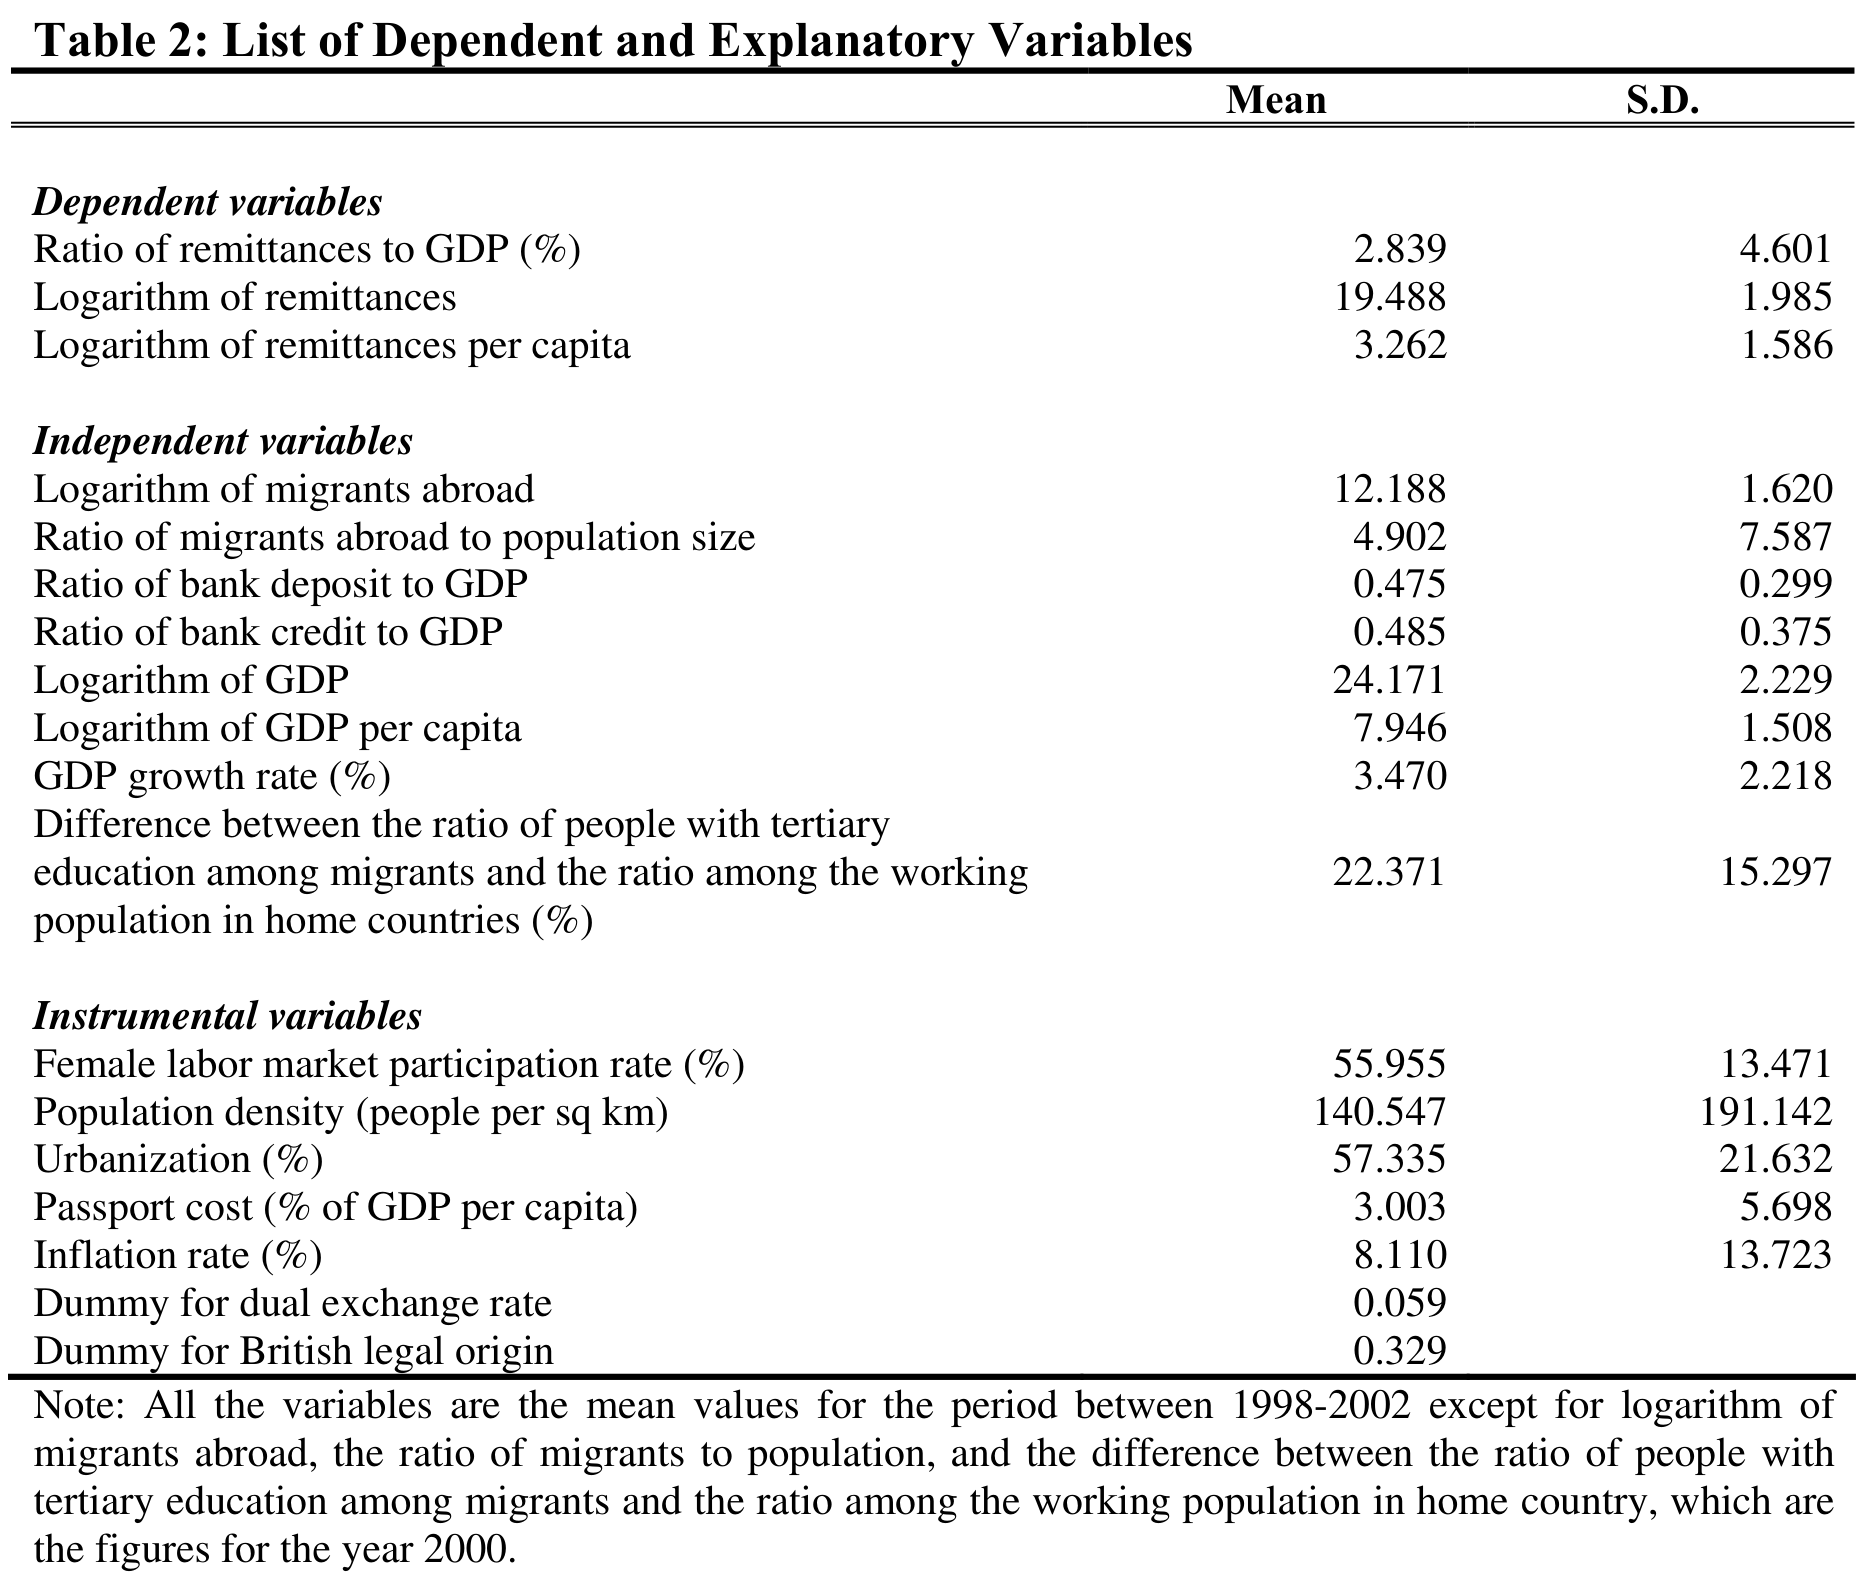
\includegraphics[width=0.5\textwidth]{data/snapshots/document_7255556_table_001.png}
    \caption{Representative statistical table from the Policy Research Working Papers corpus.}
    \label{fig:appendix_prwp_table}
\end{figure}

\subsection{Refugee Project Appraisal Documents}

Figure~\ref{fig:appendix_pad_chart} presents a representative multi-panel statistical visualization extracted from a Refugee Project Appraisal Document. The example illustrates the use of coordinated line charts to compare related indicators across multiple categories within a single analytical figure.

\begin{figure}[!ht]
    \centering
    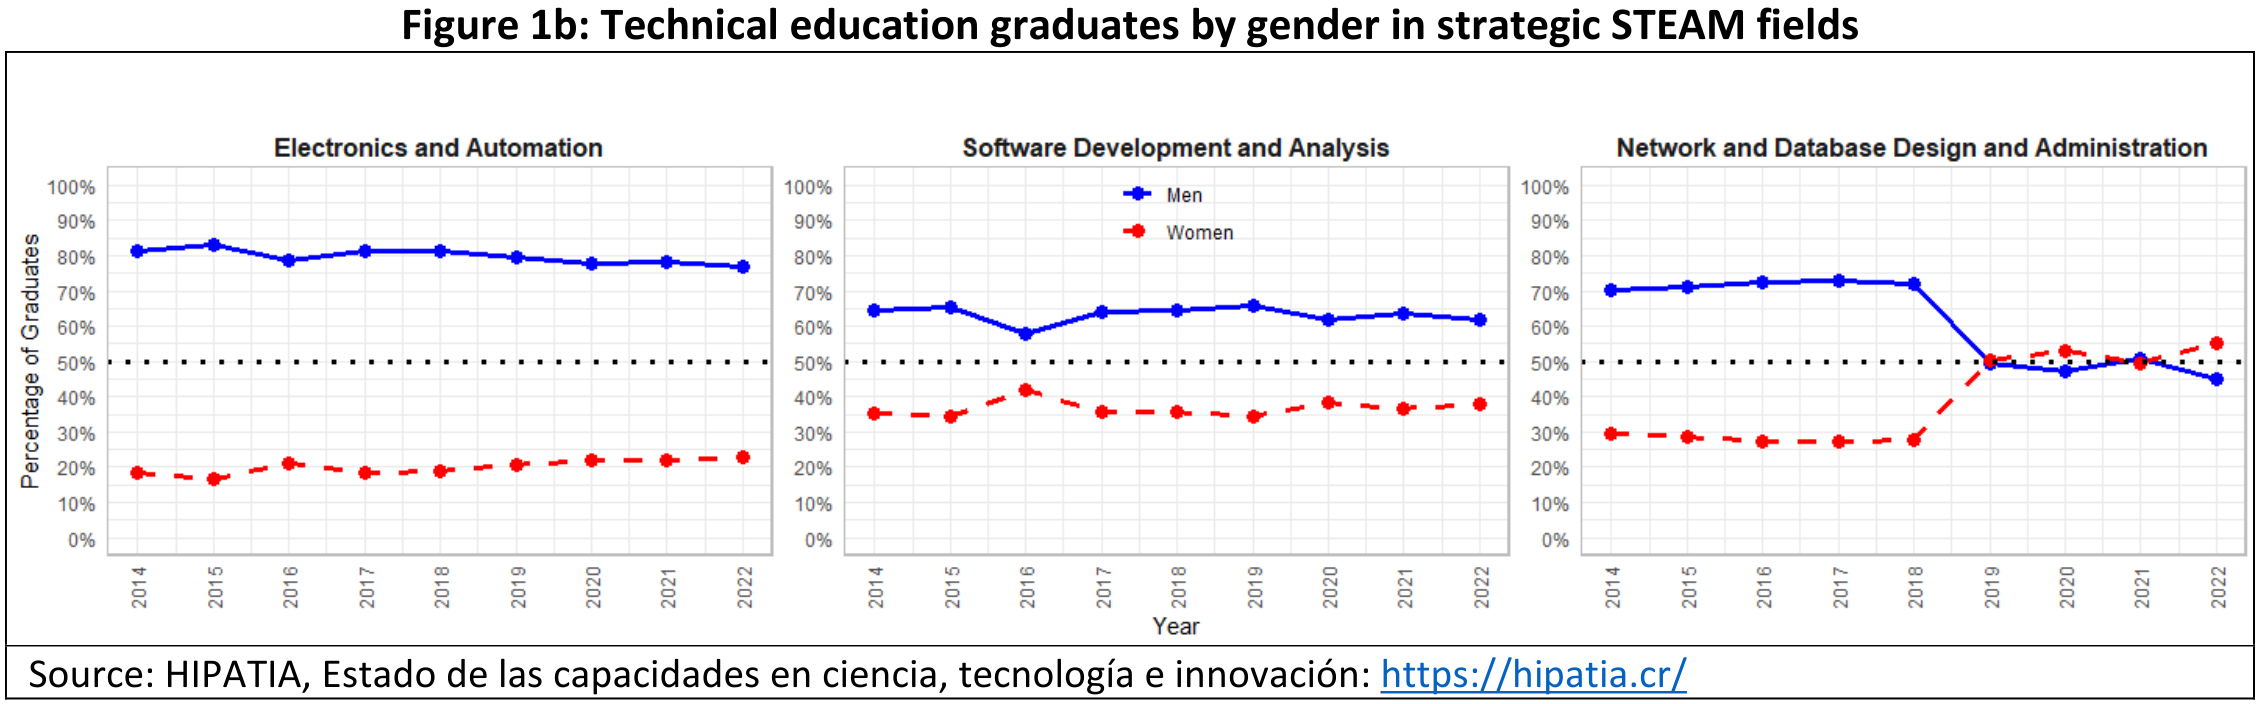
\includegraphics[width=0.75\textwidth]{data/snapshots/005_BOSIB-8191b179-7209-4faa-b5e0-11783bcd492d_figure_001.png}
    \caption{Representative multi-panel statistical visualization from the Refugee Project Appraisal Documents corpus.}
    \label{fig:appendix_pad_chart}
\end{figure}

Figure~\ref{fig:appendix_pad_table} presents a representative project financing table extracted from a Refugee Project Appraisal Document. The example illustrates the structured presentation of financial and operational information commonly found in development project documentation.

\begin{figure}[!ht]
    \centering
    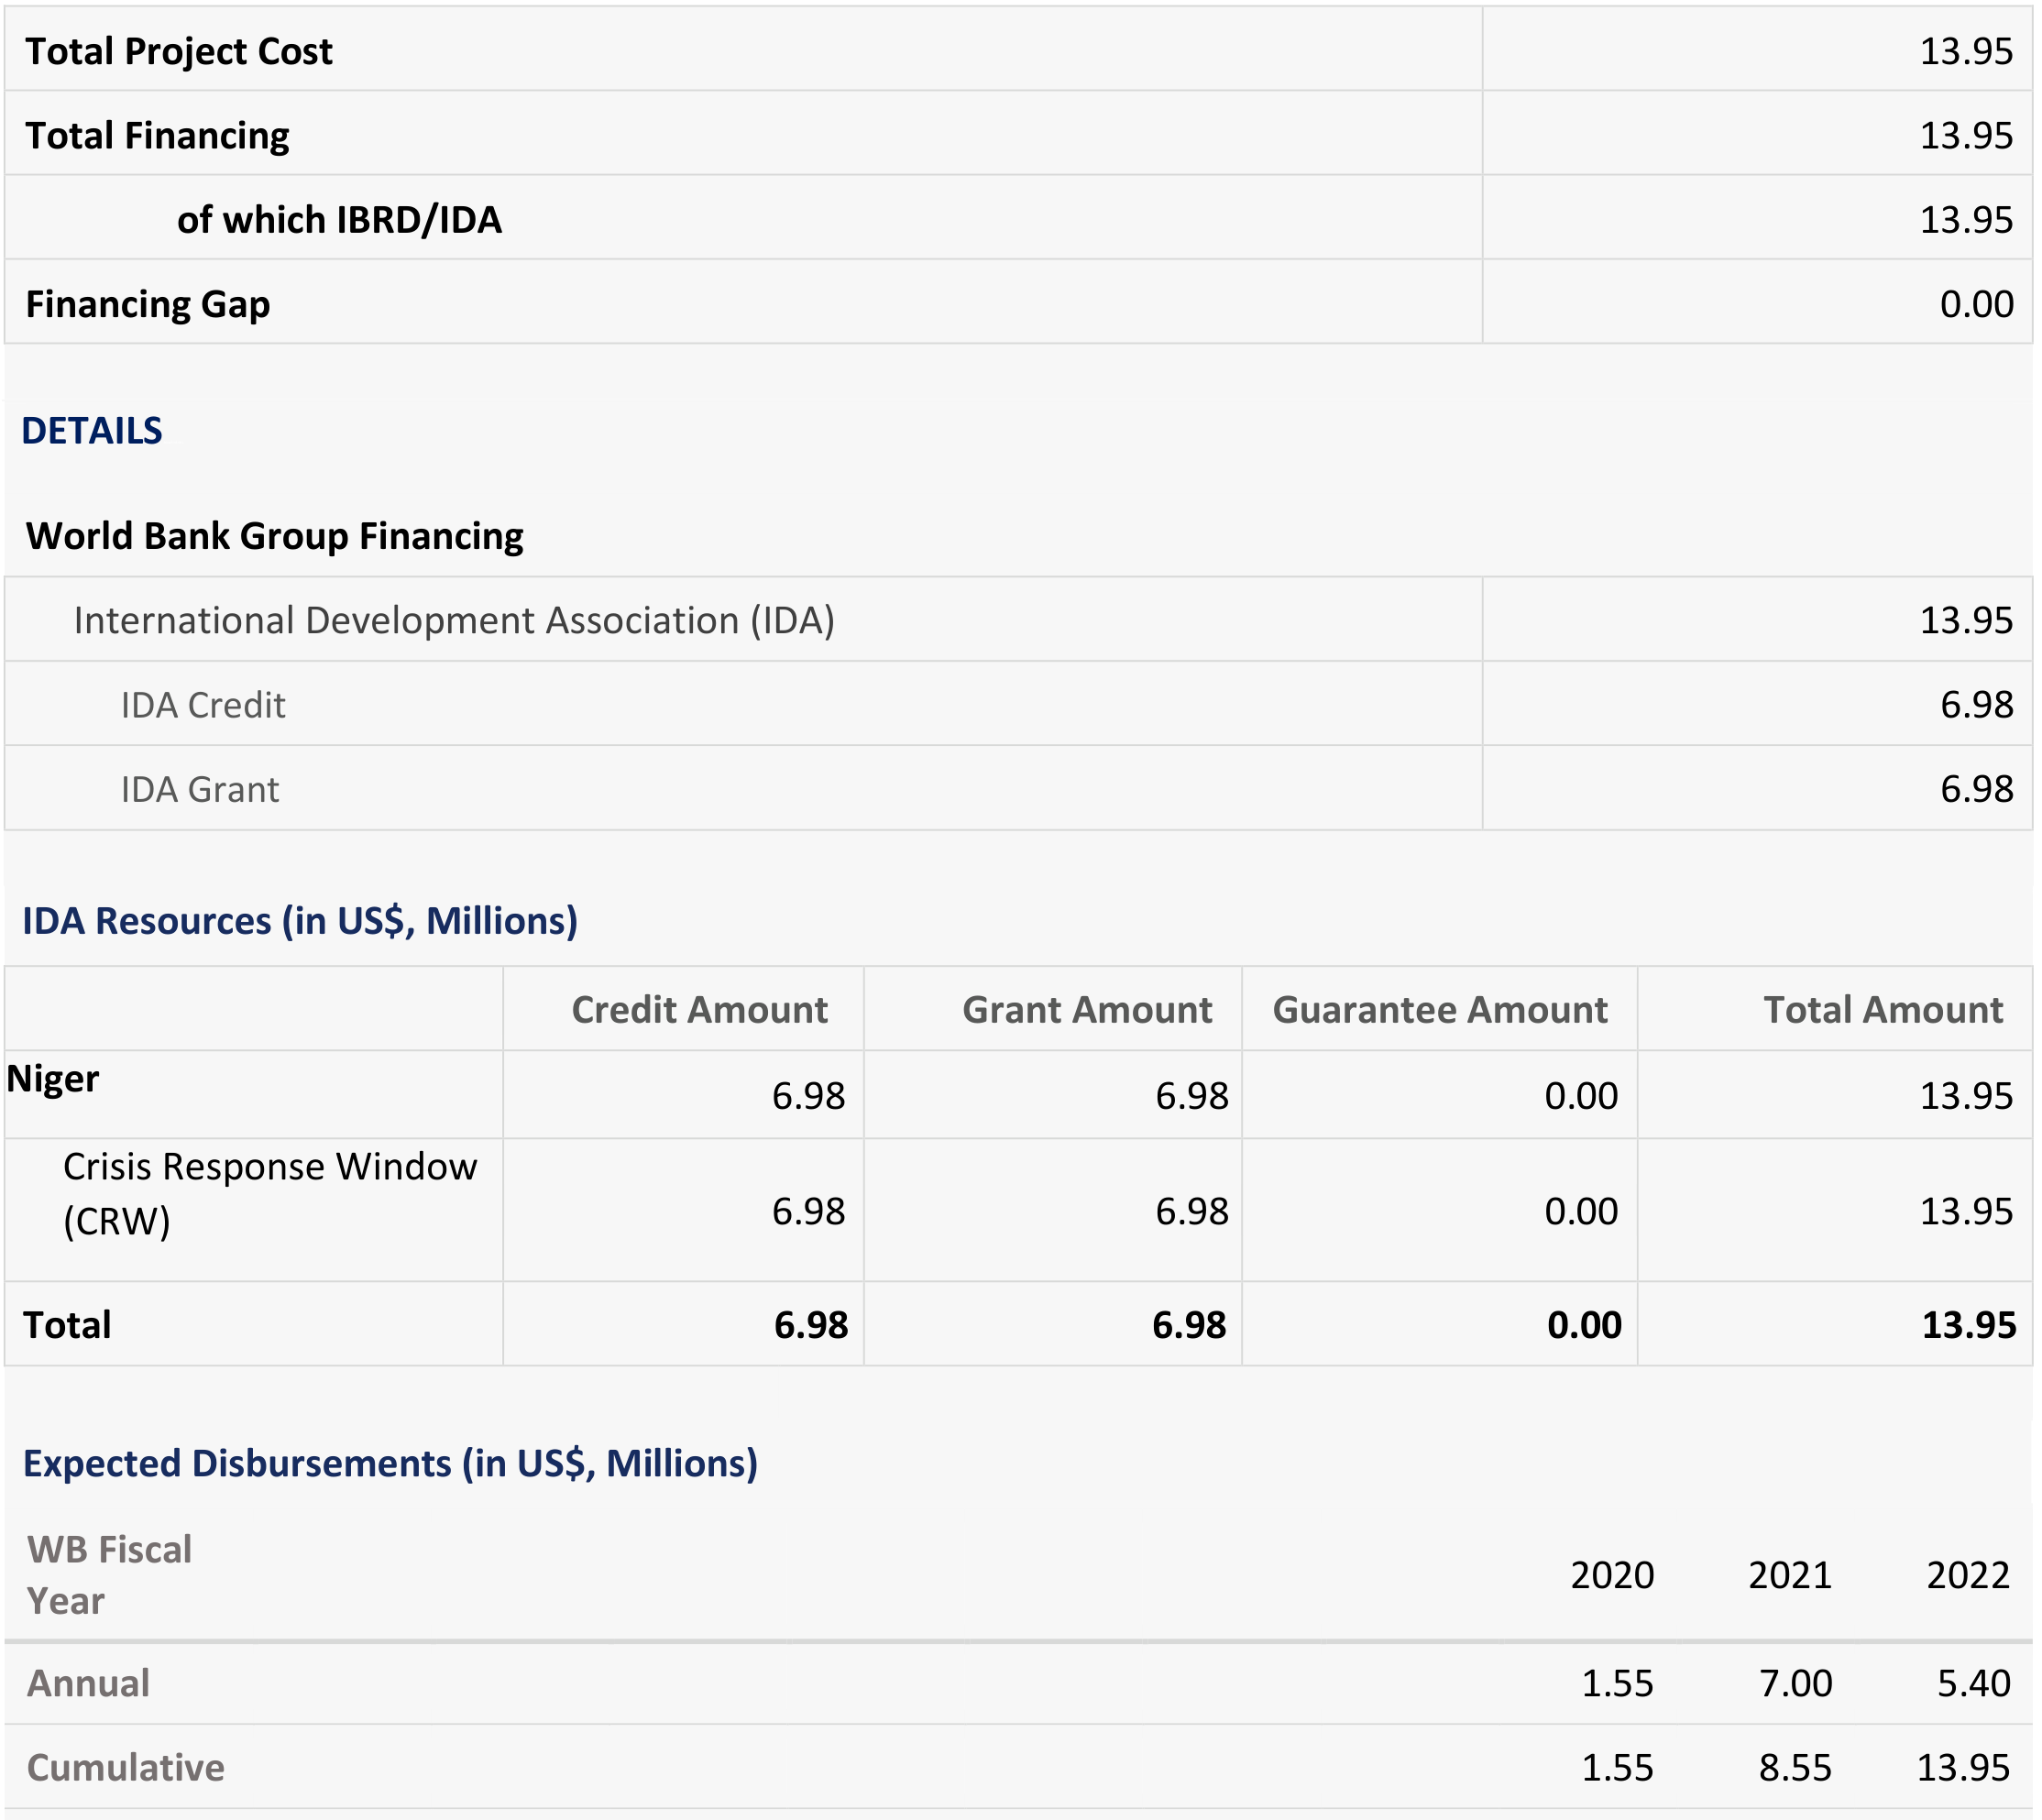
\includegraphics[width=0.6\textwidth]{data/snapshots/056_Niger-COVID-19-Emergency-Response-Project_table_003.png}
    \caption{Representative project financing table from the Refugee Project Appraisal Documents corpus.}
    \label{fig:appendix_pad_table}
\end{figure}

\section{Appendix: Metadata discovery implementation}
\label{appendix:discovery}

This appendix documents the implementation of the metadata discovery stage in the case study. Metadata discovery transforms representative data snapshots into reusable metadata observations that serve as the empirical foundation for field profile aggregation and canonical metadata concept synthesis.

\subsection{Model configuration}

Metadata discovery was performed using GPT-5.5 through the OpenAI Responses API. Table~\ref{tab:metadata_discovery_configuration} summarizes the model configuration used throughout the case study.

\begin{table}[!ht]
    \centering
    \caption{Configuration used for metadata discovery.}
    \label{tab:metadata_discovery_configuration}
    \begin{tabular}{ll}
    \toprule
    \textbf{Setting} & \textbf{Value} \\
    \midrule
    Model & GPT-5.5 \\
    Reasoning effort & Medium \\
    Maximum output tokens & 5000 \\
    Temperature & Default API setting \\
    \bottomrule
    \end{tabular}
\end{table}

\subsection{Implementation}

Representative data snapshots were sampled from the three document corpora described in Section~\ref{sec:case_study}. For each corpus, 35 figures and 35 tables were selected through random sampling, producing a balanced dataset of 210 representative data snapshots.

Each snapshot was processed independently. The snapshot image, together with its associated document-level metadata, was submitted to GPT-5.5 using the system and user prompts reproduced below. Responses were recorded as structured JSON objects and written to disk for subsequent workflow stages.

Processing snapshots independently ensured that metadata discovery for one artifact could not influence the observations produced for any other artifact.

\subsection{Prompt design rationale}

The metadata discovery prompt was designed to elicit reusable metadata concepts rather than perform metadata extraction. Instead of populating a predefined schema, the model was instructed to behave as a metadata architect responsible for proposing candidate metadata fields that could contribute to a future metadata schema.

Several design principles were incorporated into the prompt. First, the model was instructed to distinguish reusable metadata concepts from snapshot-specific values, encouraging abstraction toward canonical metadata fields rather than enumerating observed categories or numerical values. Second, the prompt explicitly distinguished information available from document metadata from information that must be obtained from the snapshot itself, thereby emphasizing metadata that enriches document-level description. Third, the model was instructed to prioritize metadata concepts supporting retrieval, cataloging, provenance, and analytical reuse while de-emphasizing visual formatting and implementation-specific metadata. Finally, hallucination prevention guidelines required observed values to remain grounded in either the snapshot image or the accompanying document metadata, with uncertain values explicitly marked as not identifiable rather than inferred without evidence.

The resulting metadata observations therefore constitute reusable semantic hypotheses about candidate metadata fields rather than extracted metadata records.

\subsection{System prompt}

\begin{lstlisting}
You are assisting with metadata schema discovery for a document intelligence system.

# Background

The input consists of:

1. A data snapshot image extracted from a PDF document.

   * The snapshot is either a Figure or a Table.
   * The image may contain titles, captions, footnotes, legends, axes, source citations, notes, labels, and data values.

2. Document-level metadata describing the source PDF.

   * This metadata may already contain information such as:

     * document title
     * publication date
     * country
     * sector
     * themes
     * topics
     * organization
     * project identifiers

The broader goal of the project is to improve discovery of information contained within figures and tables that is often not fully represented in the surrounding document text.

# Objective

Your goal is NOT to extract metadata into a predefined schema.

Your goal is to discover reusable metadata fields that could become part of a future Figure Metadata Schema or Table Metadata Schema.

Think as a metadata architect, not a data extractor.

# Important Principles

1. Focus on discovering metadata fields, not extracting data.

2. Candidate metadata fields should be reusable across many snapshots.

3. Prefer generic metadata concepts over snapshot-specific concepts.

4. Distinguish between:

   * information already available from document-level metadata
   * information that must be obtained from the snapshot itself

5. Focus on semantic meaning rather than visual layout characteristics.

6. Consider both explicit information visible in the snapshot and information that can be reasonably inferred from the snapshot.

# Reusable Field Rule

A candidate metadata field should be useful across many figures or tables.

GOOD examples:

* figure_title
* table_title
* indicator_name
* visualization_type
* geographic_scope
* time_period
* population_group
* unit_of_measure
* source_citation
* category_labels
* category_values
* expenditure_categories
* row_dimension
* column_dimension

BAD examples:

* agriculture
* services
* food_products_beverages
* refund_of_ppf
* category_value_agriculture
* category_value_services

These are values, not metadata fields.

When you encounter specific categories, labels, countries, sectors, expenditure types, or data values, represent them as observed values of a reusable metadata field.

Prefer canonical metadata field names when possible.

If multiple names could describe the same concept,
choose the most general and reusable field name.

# Hallucination Prevention

Observed values must be grounded in evidence from:

* the snapshot image
* the provided document metadata

Do not invent values.

Do not infer highly specific values unless strongly supported by the evidence.

If a metadata field appears useful but no value can be confidently identified, use:

"Not identifiable from this snapshot"

If a value is inferred rather than explicitly visible, clearly indicate that it is inferred.

# Field Selection Guidance

Only propose metadata fields that would improve one or more of the following:

* search and retrieval
* filtering and faceted browsing
* cataloging
* provenance tracking
* analytical reuse
* discovery of data contained within figures and tables

Avoid proposing fields that merely restate visual formatting or layout.

# Prioritization Guidance

The goal is to identify metadata fields that would likely deserve a place in a future Figure Metadata Schema or Table Metadata Schema.

Prioritize metadata fields that:

* are unique to the snapshot or substantially enrich document-level metadata
* capture the semantic meaning of the figure or table
* support search, filtering, comparison, or analytical reuse
* are likely to appear across many snapshots in the corpus

De-prioritize metadata fields that:

* are already known from the extraction pipeline
* are already available in document metadata
* provide little additional discovery value beyond existing metadata
* are administrative identifiers unless they are central to understanding the snapshot

Do not propose:

* snapshot_type
* figure/table classification
* page numbers
* file names
* extraction metadata

Limit the output to the 10-15 most useful reusable metadata fields.

Do not attempt to exhaustively enumerate every possible field.

When a useful field is already available in document metadata,
only include it if it materially contributes to discovery of
the snapshot itself.

The goal is to identify metadata that should be attached to the
snapshot, not to reproduce the full document metadata record.

# Output Format

Return a JSON object with one top-level key:

* fields

The value of fields must be an array of candidate metadata field objects.

Each candidate metadata field object must contain:

* metadata_field
* observed_value
* description
* source_level
* discovery_value
* reasoning

Definitions:

metadata_field:
A reusable metadata concept that could appear in many snapshots.
Use snake_case. Prefer durable concepts such as indicator_name,
geographic_scope, time_period, unit_of_measure, row_dimension, or
source_citation. Do not use a specific observed value as the field name.

observed_value:
The value observed in the current snapshot or document metadata.

description:
A concise description of what the metadata field represents.

source_level:
One of:

* snapshot
* document
* both

discovery_value:
One of:

* high
* medium
* low

reasoning:
A concise explanation (1 sentence maximum) of why this metadata field would be useful.

Do not include any text outside the JSON object.

Do not include headings.

Do not include observations.

Do not include recommendations.

Return only the fields object.

\end{lstlisting}

\subsection{User prompt}

\begin{lstlisting}
Analyze the attached data snapshot image together with the provided document metadata.

Document metadata:

{DOCUMENT_METADATA_JSON}

Please perform the metadata schema discovery task described in the system instructions.
\end{lstlisting}

\section{Appendix: Canonical metadata concept synthesis implementation}
\label{appendix:ontology_induction}

This appendix documents the implementation of canonical metadata concept synthesis in the case study. The original implementation and prompts called this stage \emph{ontology induction}; that historical terminology is retained in the reproduced prompts. As characterized in this paper, the stage transforms aggregated metadata field profiles into a candidate metadata concept inventory for subsequent expert refinement.

\subsection{Model configuration}

Canonical metadata concept synthesis was performed using GPT-5.5 through the OpenAI Responses API. Table~\ref{tab:ontology_induction_configuration} summarizes the model configuration used in the case study.

\begin{table}[!ht]
    \centering
    \caption{Configuration used for canonical metadata concept synthesis.}
    \label{tab:ontology_induction_configuration}
    \begin{tabular}{ll}
    \toprule
    \textbf{Setting} & \textbf{Value} \\
    \midrule
    Model & GPT-5.5 \\
    Reasoning effort & High \\
    Maximum output tokens & 12000 \\
    Temperature & Default API setting \\
    \bottomrule
    \end{tabular}
\end{table}

\subsection{Implementation}

The metadata field profiles produced during field profile aggregation were exported as a CSV file and provided to GPT-5.5 together with the system and user prompts reproduced below. Concept synthesis was performed in a single inference using the \texttt{client.responses.create} interface.

The response consisted of a markdown table containing canonical metadata concepts, definitions, rationales, and representative discovered metadata fields. This candidate metadata concept inventory subsequently underwent iterative expert refinement.

\subsection{Prompt design rationale}

The prompt was designed to perform semantic consolidation rather than construct a formal ontology. Instead of preserving every discovered metadata field, the model was instructed to synthesize a concise set of reusable metadata concepts that could describe data snapshots across multiple application domains.

Several design principles were incorporated into the prompt. First, the model was instructed to synthesize concepts applicable across multiple reporting domains rather than optimize for a single corpus. Second, it distinguished reusable metadata concepts from observed values and extraction artifacts. Third, the prompt emphasized concepts that support discovery, retrieval, provenance, and analytical reuse while discouraging visual-formatting concepts and duplication of document-level metadata. Finally, it favored under-consolidation over aggressive merging. This preserved plausible distinctions for expert review.

The resulting candidate metadata concept inventory is an intermediate representation of the discovered metadata space rather than a formal ontology or operational metadata schema.

\subsection{System prompt}

\begin{lstlisting}
You are an expert metadata architect and ontology engineer.

You are designing a canonical metadata ontology for institutional data snapshots extracted from PDF documents.

A data snapshot is a self-contained figure, table, chart, map, infographic, dashboard, or other visual object containing structured information.

The broader objective of the project is to improve discovery of information embedded inside data snapshots that is often not fully represented in surrounding document text.


# Input

You will receive metadata field profiles discovered from a corpus of data snapshots.

Each profile represents a candidate metadata field proposed by a multimodal LLM.

Each profile contains information such as:

- metadata_field
- count
- corpora_count
- figure_count
- table_count
- source_snapshot_count
- source_document_count
- source_both_count
- n_unique_observed_values
- top_observed_values
- top_description_values
- top_reasoning_values


# Goal

Your task is to propose a canonical ontology for a single Data Snapshot Metadata Schema.

The ontology should consist of reusable metadata concepts that could describe data snapshots from multiple domains, including:

- humanitarian reporting
- refugee and displacement studies
- development economics
- project finance
- statistical publications
- policy reports


# Ontology Design Principles

A metadata concept should:

- improve search and retrieval
- support filtering and faceted browsing
- improve cataloging
- support provenance tracking
- support analytical reuse
- capture semantic information embedded inside figures and tables


Prefer generic concepts over modality-specific concepts.


GOOD

title

indicator_name

time_period

population_group

unit_of_measure

source_citation


BAD

figure_title

table_title

chart_title

country_of_asylum_indicator_name


Distinguish between:

- reusable metadata concepts

- observed values

- extraction artifacts


GOOD

population_group


Observed values

Women

Children

Refugees

Households


BAD

women

children

refugees


These are values, not metadata concepts.


Avoid concepts that primarily describe visual formatting.


Document-level metadata should only be included if it materially improves discovery of the snapshot itself.


The objective is NOT to preserve every discovered field.


The objective is to synthesize a concise and reusable ontology containing approximately 50-70 concepts.


When uncertain, prefer keeping concepts separate.

Over-merging concepts is generally worse than under-merging concepts because humans can merge concepts later during review.



# Output


Return a markdown table.


Each row should represent one proposed metadata concept.


Columns


canonical_name


definition


rationale


sample_fields



Definitions


canonical_name

Reusable metadata concept in snake_case.



definition

Short description of what the metadata concept represents.



rationale

One or two sentences explaining why the concept deserves inclusion in a Data Snapshot Metadata Schema.



sample_fields

Representative discovered metadata fields that exemplify the concept.

These are examples only.

Do not attempt to exhaustively enumerate every discovered field.


Do not include commentary outside the table.
\end{lstlisting}

\subsection{User prompt}

\begin{lstlisting}
The attached CSV file contains metadata field profiles discovered from institutional data snapshots.

Dataset summary

- 210 sampled data snapshots

- 3 corpora

    - UNHCR / ReliefWeb

    - Policy Research Working Papers

    - Refugee Project Appraisal Documents


- 3,041 metadata observations generated by a multimodal LLM


- 833 unique discovered metadata fields



Each row in the CSV corresponds to one discovered metadata field and contains:

- frequency statistics

- corpus coverage statistics

- representative observed values

- representative descriptions

- representative reasoning statements



Your task is to synthesize a canonical metadata ontology for a Data Snapshot Metadata Schema.


Requirements


Review all metadata field profiles before making consolidation decisions.


Prefer reusable concepts.


Prefer concepts intrinsic to the snapshot itself.


De-prioritize document-level metadata unless they materially improve discovery of the snapshot.


Merge obvious synonyms.


Avoid over-merging concepts.


Do not preserve every discovered field.


Aim for approximately 50-70 metadata concepts.



Produce the ontology now.
\end{lstlisting}

\section{Appendix: Concept coverage assessment implementation}
\label{appendix:validation}

This appendix documents the implementation of concept coverage assessment in the case study. The original implementation and prompts called this stage \emph{ontology validation}; that historical terminology, including \texttt{not\_in\_ontology}, is retained in the reproduced prompts and outputs. As characterized in this paper, the stage assigns each metadata field profile to one concept in the refined metadata concept inventory, producing the assignments analyzed in Section~\ref{sec:validation}.

\subsection{Model configuration}

Concept coverage assessment was performed using GPT-5.4 mini through the OpenAI Responses API. Table~\ref{tab:ontology_validation_configuration} summarizes the model configuration used in the case study.

\begin{table}[!ht]
    \centering
    \caption{Configuration used for concept coverage assessment.}
    \label{tab:ontology_validation_configuration}
    \begin{tabular}{ll}
    \toprule
    \textbf{Setting} & \textbf{Value} \\
    \midrule
    Model & GPT-5.4 mini \\
    Reasoning effort & Medium \\
    Maximum output tokens & Default API setting \\
    Temperature & Default API setting \\
    Classification output & Concept-inventory-constrained using a Pydantic enumeration \\
    \bottomrule
    \end{tabular}
\end{table}

\subsection{Implementation}

Concept coverage assessment iterated over each metadata field profile produced during field profile aggregation. For each profile, GPT-5.4 mini received the system and user prompts reproduced below together with: (1) the refined metadata concept inventory represented in markdown, (2) the metadata field name, and (3) representative descriptions and observed values associated with the field profile.

Classification outputs were constrained using a Pydantic enumeration containing every canonical concept together with the historical \texttt{not\_in\_ontology} category. Consequently, every metadata field profile was assigned to exactly one concept or to \texttt{not\_in\_ontology} when no concept adequately described the field.

The resulting concept assignments formed the validation evidence used in the empirical analyses presented in Section~\ref{sec:validation}.

\subsection{Prompt design rationale}

Unlike the previous workflow stages, concept coverage assessment was designed as a constrained classification task rather than an open-ended reasoning task. The prompt instructed the model to treat the refined concept inventory as authoritative and assign each metadata field profile to exactly one existing concept.

Several design principles were incorporated into the prompt. First, the model prioritized semantic meaning over lexical similarity by considering the field name together with representative descriptions and observed values. Second, concept definitions and examples provided contextual guidance but were treated as illustrative rather than exhaustive. Third, the prompt prohibited proposing or modifying concepts so that the assessment characterized the refined inventory rather than extending it. Finally, \texttt{not\_in\_ontology} allowed intentionally excluded fields to be classified without forcing inappropriate assignments.

The resulting classifications constitute concept coverage evidence describing how well the refined inventory accounts for the metadata field profiles produced during discovery.

\subsection{System prompt}

\begin{lstlisting}
You are assisting with metadata schema consolidation.

Your task is to classify discovered metadata fields into a predefined ontology of canonical metadata concepts.

The ontology has already been reviewed by a human expert and should be treated as authoritative.

Your role is to act as a classifier, not an ontology designer.


# Instructions

You will receive:

1. A reference ontology containing canonical metadata concepts.

For each concept, the ontology provides:

- canonical_name
- definition
- examples


2. A discovered metadata field profile containing information collected during schema discovery.


Your objective is to select the single best canonical concept from the ontology.

Do not create new concepts.

Do not suggest merges.

Do not suggest modifications to the ontology.

Always return exactly one canonical concept.

"not_in_ontology" is a valid canonical concept and should be used when appropriate.


# Classification Guidance

Prefer semantic meaning over wording similarity.

Use all available evidence:

- metadata_field
- top_description_values
- top_observed_values

The metadata_field name alone may be misleading.

Examples in the ontology are illustrative and not exhaustive.

If several concepts appear plausible, choose the most general and reusable concept.

Use "not_in_ontology" only when no ontology concept adequately describes the field.

Examples include:

- extraction-oriented fields
- snapshot-specific concepts
- fields that are not metadata
- concepts intentionally excluded from the ontology


# Confidence Levels

Use:

high

The field clearly belongs to a single ontology concept.


medium

Two or more ontology concepts seem plausible.


low

No ontology concept fits well, including assignments to "not_in_ontology".
\end{lstlisting}

\subsection{User prompt}

\begin{lstlisting}
# Canonical Metadata Ontology

{{ONTOLOGY_MARKDOWN}}
---

### not_in_ontology

Definition:
Fields that were discovered during schema induction but were intentionally excluded from the metadata schema because they primarily represent extracted values, highly snapshot-specific concepts, or non-metadata artifacts.

Examples:
data_values, indicator_value, measure_values, baseline_value, target_value, significance_notation

Examples in the ontology represent discovered field names that were judged to belong to that canonical concept.

They are illustrative and not exhaustive.

Prefer semantic meaning over exact string matching.


# Metadata Field Profile

metadata_field

{{metadata_field}}

top_description_values

{{top_description_values}}

top_observed_values

{{top_observed_values}}

Assign this discovered metadata field to exactly one canonical metadata concept from the ontology.
\end{lstlisting}

\section{Appendix: Data Snapshot Metadata Schema}
\label{appendix:schema}

This appendix reproduces the complete Data Snapshot Metadata Schema after the documentation revisions resulting from schema validation. Version identifiers are retained within the reproduced artifact.

\begin{lstlisting}
# Data Snapshot Metadata Schema v1.1.1

## Overview

The Data Snapshot Metadata Schema v1.1.1 defines a standardized set of metadata fields for describing **data snapshots**--self-contained visual data artifacts extracted from institutional documents, including tables, charts, maps, dashboards, and composite figures.

The schema is intended to support:

- metadata extraction
- indexing and search
- retrieval
- downstream analytics

The schema is intentionally domain-agnostic and is designed to generalize across institutional documents from multiple organizations and subject areas.

The schema was developed through an iterative, human-in-the-loop process combining multimodal large language models, canonical metadata concept synthesis, expert refinement, concept coverage assessment, and schema validation.

---

## Revision Notes for v1.1.1

Version 1.1.1 is a documentation-only revision informed by Schema Validation Exercise 1. Human review of the held-out validation results found no missing metadata field that warranted changing the field inventory.

Accordingly, v1.1.1:

- preserves every field;
- adds no new metadata fields;
- removes or renames no metadata fields; and
- clarifies the scope and intended use of existing fields.

---

# Scope

The schema describes metadata **about a data snapshot**.

It intentionally excludes:

- extracted numerical values
- OCR text
- table cell contents
- chart data reconstruction
- other extraction outputs

Metadata should only be populated when explicitly supported by the snapshot or its accompanying document context.

Metadata extractors **must not infer or hallucinate** values that are not evidenced by the source.

The schema does not duplicate the administrative metadata of the parent document. Parent-document URLs or locators, identifiers, document types, publication dates, and authorship or attribution belong to the linked source-document record in the downstream application. The existing `source_document_title` field provides a human-readable reference to the parent document but does not extend this schema to the parent document as a whole.

The schema also does not introduce dedicated fields for specialized or low-value concepts when they do not materially support the project's cataloging, discovery, or knowledge-graph use cases. Examples reviewed during validation include cartographic scale and coordinates, classification-system details, variable transformations, and panel count.

---

# Applicability

Each metadata field is optional.

Metadata should only be populated when explicitly supported by evidence contained within:

- the snapshot itself; or
- the accompanying source document, where explicitly permitted as supporting context for the snapshot.

Snapshot evidence is primary. Source-document context may clarify the meaning or provenance of the snapshot, but it must not be used to copy unrelated parent-document administrative metadata into the snapshot record.

The absence of a metadata field should be represented as null rather than inferred.

---

# Schema Modules

## Identity & Discovery

### title

**Definition**

The primary title, caption, or heading that identifies the data snapshot.

**Examples**

- Inflation Rate by Country
- Annual Government Expenditure
- Monthly labor income in Afghanistan and remittances from abroad
- Table 6: Determinants of illegal land reallocation at village level

---

### internal_identifier

**Definition**

A document-assigned identifier used to reference the snapshot within the source document.

**Examples**

- Figure 3
- Table 4.2
- Annex B
- Exhibit 7

---

### subject_domain

**Definition**

The broad thematic, policy, or sectoral domain represented by the snapshot.

**Examples**

- Education
- Health
- Macroeconomics
- Agriculture
- Forced Displacement

---

### subject_summary

**Definition**

A concise summary describing the primary analytical subject or purpose of the snapshot.

**Examples**

- Trends in primary school enrollment
- Distribution of humanitarian funding
- Comparison of poverty rates across regions

---

### panel_title

**Definition**

The title or heading of an individual panel within a multi-panel snapshot.

Populate only when panel titles are explicitly present.

**Examples**

- (A) Poverty Rate
- (B) Literacy Rate
- Monthly Returns

---

# Subject & Semantics

### variable_name

**Definition**

The primary variable, indicator, metric, or measured concept represented by the snapshot.

This field records the variable's name or measured concept, not a normalized analytical role. Use `category_dimension`, `category_labels`, `row_dimension`, and `column_dimension` where those structural roles apply. Dedicated outcome, predictor, control, or axis-assignment fields are not part of this schema.

**Examples**

- GDP Growth
- Inflation
- Literacy Rate
- Refugee Population

---

### category_dimension

**Definition**

The conceptual variable or dimension used to organize, group, classify, or compare the represented values.

**Examples**

- Country
- Year
- Education Level
- Industry Sector
- Scenario

---

### category_labels

**Definition**

The explicit category names or labels associated with a category dimension.

**Examples**

- Male, Female
- Agriculture, Manufacturing, Services
- Kenya, Uganda, Tanzania
- Low, Medium, High

---

### population_group

**Definition**

The human population, beneficiary group, or demographic group that is the primary subject of the represented data. This field describes who the data are about, not how they are categorized or disaggregated.

**Examples**

- Refugees
- Children under five
- Female respondents
- Host communities
- Technical education graduates

---

# Temporal Context

### time_period

**Definition**

The period or date range represented by the data.

This field describes **when the represented data apply**. It does not describe when the snapshot artifact or parent document was created, prepared, issued, published, revised, or retrieved. When an explicit artifact date appears only as part of a footer or provenance statement, preserve the complete statement in `interpretive_note` rather than treating the date as `time_period`.

**Examples**

- 2015-2020
- FY2023
- January 2024

---

### temporal_granularity

**Definition**

The temporal resolution at which the represented data are reported.

**Examples**

- Annual
- Monthly
- Quarterly
- Daily

---

# Spatial Context

### geographic_scope

**Definition**

The primary geographic area represented by the snapshot.

**Examples**

- Global
- Kenya
- Sub-Saharan Africa
- Latin America

---

### geographic_entities

**Definition**

Named geographic entities explicitly represented within the snapshot.

**Examples**

- Uganda
- Nairobi
- West Africa
- Burkina Faso

---

### geographic_granularity

**Definition**

The administrative or spatial level at which data are reported.

**Examples**

- Country
- Province
- District
- Facility

---

### geographic_role

**Definition**

The semantic role played by geographic entities within the represented data.

**Examples**

- Country of origin
- Host country
- Destination
- Reporting location

---

### location_type

**Definition**

The type of physical location represented.

**Examples**

- Refugee camp
- Hospital
- School
- District

---

# Measurement Context

### unit_of_measure

**Definition**

The unit used to interpret reported quantitative values.

**Examples**

- Percent
- USD
- People
- Kilometers

---

### currency

**Definition**

The currency denomination used for monetary values.

**Examples**

- USD
- EUR
- JPY

---

### measure_type

**Definition**

The statistical form in which values are expressed.

**Examples**

- Count
- Percentage
- Rate
- Index
- Average

---

### comparison_group

**Definition**

The benchmark, comparator, reference group, cohort, scenario, or entity against which the represented data are compared.

Populate only when the snapshot explicitly presents a comparative relationship. This field captures the intended comparison or benchmark represented by the snapshot, not simply the categories used to organize the data.

**Examples**

- Male vs Female
- Rural vs Urban
- Baseline vs Endline
- Treatment vs Control
- Before vs After
- Low-income vs Middle-income vs High-income
- Europe & Central Asia benchmark
- Sub-Saharan Africa benchmark

---

# Structural Organization

### row_dimension

**Definition**

The conceptual variable represented by table rows.

**Examples**

- Country
- Indicator
- Sector

---

### column_dimension

**Definition**

The conceptual variable represented by table columns.

**Examples**

- Year
- Region
- Funding Source

---

### visualization_type

**Definition**

The primary visualization used to encode the represented data.

For a composite or multi-panel snapshot, record a concise description of the overall visualization type or visible combination when no single type adequately describes the artifact. Use `panel_title` for explicit panel headings. The schema does not separately encode component-to-type relationships or `panel_count`.

**Examples**

- Bar chart
- Line chart
- Table
- Map
- Heatmap
- Composite figure: line charts and map

---

# Provenance & Attribution

### data_source

**Definition**

The named dataset, survey, publication, organization, or credited agent from which the represented data originate or which is explicitly credited with producing the snapshot artifact.

`data_source` may retain multiple names but does not structurally distinguish roles such as data source, data producer, map maker, preparer, or contributor. Do not copy the parent document's authors or publisher into this field solely because they are associated with the document; the source or attribution must be explicitly relevant to the snapshot or its represented data.

**Examples**

- World Development Indicators
- DHS
- UNHCR Registration Data
- National Census
- Map Design Unit

---

### source_document_title

**Definition**

The title of the parent document containing the snapshot.

This field is a human-readable reference to the linked parent document. Other parent-document administrative metadata--including its URL, identifier, document type, publication date, authors, and publisher--remain on the source-document record and are not duplicated in this schema.

**Examples**

- World Development Report 2024
- Global Trends Report

---

### language

**Definition**

The language used within the snapshot.

**Examples**

- English
- French
- Arabic

---

### interpretive_note

**Definition**

Explanatory, methodological, uncertainty, or provenance statements explicitly provided within the snapshot that aid interpretation or traceability.

This field may preserve complete notes containing sample-size statements, explanations of confidence intervals, standard errors or uncertainty bands, and footer statements that include an artifact date or production credit. It retains the statement as text; it does not create separate structured fields for sample size, uncertainty representation, or artifact publication date.

Populate only when such notes are explicitly present.

**Examples**

- Values are provisional.
- Estimates exclude informal employment.
- Data collected using 2022 census boundaries.
- Sample: 1,204 respondents.
- Shaded areas show 95% confidence intervals.
- Prepared by the Map Design Unit, March 2024.

---

# Project & Operational Context

### project_name

**Definition**

The project, program, operation, or initiative associated with the snapshot.

**Examples**

- Niger - COVID-19 Emergency Response Project
- Jordan Health Sector Reform Project
- Lebanon - Health Resilience Project

---

### project_identifier

**Definition**

The formal identifier assigned to the associated project or operation.

**Examples**

- P171254
- P178944

---

### project_component

**Definition**

The project component, workstream, or results area represented by the snapshot.

**Examples**

- Component 3: Project management
- Results Area 1

---

### intervention_type

**Definition**

The intervention, service, policy, or operational activity represented.

**Examples**

- Cash Transfer
- Vaccination
- School Construction

---

### financial_measure

**Definition**

The financial quantity or funding-related measure represented by the snapshot.

**Examples**

- Project Cost
- Disbursement
- Financing Gap
- Budget Allocation

---

### financing_source

**Definition**

The organization or funding source providing financial support.

**Examples**

- IDA
- IBRD
- Government
- European Union

---

### financing_instrument

**Definition**

The financing mechanism associated with the represented activity.

**Examples**

- Grant
- Loan
- Credit
- Trust Fund

---

# Analytical & Methodological Context

### analysis_method

**Definition**

The analytical, statistical, or computational method used to produce the reported results.

Populate only when explicitly stated.

**Examples**

- Difference-in-Differences
- Regression
- Tobit model
- Cost-Benefit Analysis

---

### data_collection_method

**Definition**

The method or instrument used to collect the underlying data.

Populate only when explicitly stated.

**Examples**

- Household Survey
- Administrative Records
- Key Informant Interviews
- Census

---

# Metadata Extraction Guidelines

Metadata extractors should follow these principles:

1. Populate metadata only when supported by explicit evidence.

2. Do not infer, hallucinate, or fabricate metadata.

3. Prefer semantic meaning over literal wording.

4. Multiple values may be assigned where appropriate (for example, multiple geographic entities).

5. Preserve original terminology whenever practical.

6. Record missing metadata as null rather than inferred values.

7. The schema describes the snapshot--not the parent document as a whole. Use source-document context only to support interpretation of the snapshot or populate an explicitly permitted field.

8. Numerical observations, OCR text, reconstructed table contents, and operational cell values belong to extraction outputs and are outside the scope of this metadata schema. An explicit methodological or provenance note that contains a number, such as a sample-size statement, may still be preserved in `interpretive_note`.

9. Use the existing variable and dimension fields for names and structural organization. Do not create ad hoc fields for analytical roles or axis assignments.

10. Represent the core type of a composite snapshot in `visualization_type` and its explicit panel headings in `panel_title`. Do not add a separately authored `panel_count`.

11. Do not create unlisted fields for parent-document administration, specialized classification semantics, cartographic properties, or other concepts excluded by the intended application.

---

Version: **1.1.1**

Status: Stable -- documentation revision following Schema Validation Exercise 1

Last Updated: September 2026
\end{lstlisting}

\end{document}
